% Options for packages loaded elsewhere
\PassOptionsToPackage{unicode}{hyperref}
\PassOptionsToPackage{hyphens}{url}
%
\documentclass[
]{book}
\usepackage{amsmath,amssymb}
\usepackage{lmodern}
\usepackage{iftex}
\ifPDFTeX
  \usepackage[T1]{fontenc}
  \usepackage[utf8]{inputenc}
  \usepackage{textcomp} % provide euro and other symbols
\else % if luatex or xetex
  \usepackage{unicode-math}
  \defaultfontfeatures{Scale=MatchLowercase}
  \defaultfontfeatures[\rmfamily]{Ligatures=TeX,Scale=1}
\fi
% Use upquote if available, for straight quotes in verbatim environments
\IfFileExists{upquote.sty}{\usepackage{upquote}}{}
\IfFileExists{microtype.sty}{% use microtype if available
  \usepackage[]{microtype}
  \UseMicrotypeSet[protrusion]{basicmath} % disable protrusion for tt fonts
}{}
\makeatletter
\@ifundefined{KOMAClassName}{% if non-KOMA class
  \IfFileExists{parskip.sty}{%
    \usepackage{parskip}
  }{% else
    \setlength{\parindent}{0pt}
    \setlength{\parskip}{6pt plus 2pt minus 1pt}}
}{% if KOMA class
  \KOMAoptions{parskip=half}}
\makeatother
\usepackage{xcolor}
\IfFileExists{xurl.sty}{\usepackage{xurl}}{} % add URL line breaks if available
\IfFileExists{bookmark.sty}{\usepackage{bookmark}}{\usepackage{hyperref}}
\hypersetup{
  pdftitle={06-ESTACIONARIEDAD},
  pdfauthor={Emiliano Pérez Caullieres},
  hidelinks,
  pdfcreator={LaTeX via pandoc}}
\urlstyle{same} % disable monospaced font for URLs
\usepackage{color}
\usepackage{fancyvrb}
\newcommand{\VerbBar}{|}
\newcommand{\VERB}{\Verb[commandchars=\\\{\}]}
\DefineVerbatimEnvironment{Highlighting}{Verbatim}{commandchars=\\\{\}}
% Add ',fontsize=\small' for more characters per line
\usepackage{framed}
\definecolor{shadecolor}{RGB}{248,248,248}
\newenvironment{Shaded}{\begin{snugshade}}{\end{snugshade}}
\newcommand{\AlertTok}[1]{\textcolor[rgb]{0.94,0.16,0.16}{#1}}
\newcommand{\AnnotationTok}[1]{\textcolor[rgb]{0.56,0.35,0.01}{\textbf{\textit{#1}}}}
\newcommand{\AttributeTok}[1]{\textcolor[rgb]{0.77,0.63,0.00}{#1}}
\newcommand{\BaseNTok}[1]{\textcolor[rgb]{0.00,0.00,0.81}{#1}}
\newcommand{\BuiltInTok}[1]{#1}
\newcommand{\CharTok}[1]{\textcolor[rgb]{0.31,0.60,0.02}{#1}}
\newcommand{\CommentTok}[1]{\textcolor[rgb]{0.56,0.35,0.01}{\textit{#1}}}
\newcommand{\CommentVarTok}[1]{\textcolor[rgb]{0.56,0.35,0.01}{\textbf{\textit{#1}}}}
\newcommand{\ConstantTok}[1]{\textcolor[rgb]{0.00,0.00,0.00}{#1}}
\newcommand{\ControlFlowTok}[1]{\textcolor[rgb]{0.13,0.29,0.53}{\textbf{#1}}}
\newcommand{\DataTypeTok}[1]{\textcolor[rgb]{0.13,0.29,0.53}{#1}}
\newcommand{\DecValTok}[1]{\textcolor[rgb]{0.00,0.00,0.81}{#1}}
\newcommand{\DocumentationTok}[1]{\textcolor[rgb]{0.56,0.35,0.01}{\textbf{\textit{#1}}}}
\newcommand{\ErrorTok}[1]{\textcolor[rgb]{0.64,0.00,0.00}{\textbf{#1}}}
\newcommand{\ExtensionTok}[1]{#1}
\newcommand{\FloatTok}[1]{\textcolor[rgb]{0.00,0.00,0.81}{#1}}
\newcommand{\FunctionTok}[1]{\textcolor[rgb]{0.00,0.00,0.00}{#1}}
\newcommand{\ImportTok}[1]{#1}
\newcommand{\InformationTok}[1]{\textcolor[rgb]{0.56,0.35,0.01}{\textbf{\textit{#1}}}}
\newcommand{\KeywordTok}[1]{\textcolor[rgb]{0.13,0.29,0.53}{\textbf{#1}}}
\newcommand{\NormalTok}[1]{#1}
\newcommand{\OperatorTok}[1]{\textcolor[rgb]{0.81,0.36,0.00}{\textbf{#1}}}
\newcommand{\OtherTok}[1]{\textcolor[rgb]{0.56,0.35,0.01}{#1}}
\newcommand{\PreprocessorTok}[1]{\textcolor[rgb]{0.56,0.35,0.01}{\textit{#1}}}
\newcommand{\RegionMarkerTok}[1]{#1}
\newcommand{\SpecialCharTok}[1]{\textcolor[rgb]{0.00,0.00,0.00}{#1}}
\newcommand{\SpecialStringTok}[1]{\textcolor[rgb]{0.31,0.60,0.02}{#1}}
\newcommand{\StringTok}[1]{\textcolor[rgb]{0.31,0.60,0.02}{#1}}
\newcommand{\VariableTok}[1]{\textcolor[rgb]{0.00,0.00,0.00}{#1}}
\newcommand{\VerbatimStringTok}[1]{\textcolor[rgb]{0.31,0.60,0.02}{#1}}
\newcommand{\WarningTok}[1]{\textcolor[rgb]{0.56,0.35,0.01}{\textbf{\textit{#1}}}}
\usepackage{longtable,booktabs,array}
\usepackage{calc} % for calculating minipage widths
% Correct order of tables after \paragraph or \subparagraph
\usepackage{etoolbox}
\makeatletter
\patchcmd\longtable{\par}{\if@noskipsec\mbox{}\fi\par}{}{}
\makeatother
% Allow footnotes in longtable head/foot
\IfFileExists{footnotehyper.sty}{\usepackage{footnotehyper}}{\usepackage{footnote}}
\makesavenoteenv{longtable}
\usepackage{graphicx}
\makeatletter
\def\maxwidth{\ifdim\Gin@nat@width>\linewidth\linewidth\else\Gin@nat@width\fi}
\def\maxheight{\ifdim\Gin@nat@height>\textheight\textheight\else\Gin@nat@height\fi}
\makeatother
% Scale images if necessary, so that they will not overflow the page
% margins by default, and it is still possible to overwrite the defaults
% using explicit options in \includegraphics[width, height, ...]{}
\setkeys{Gin}{width=\maxwidth,height=\maxheight,keepaspectratio}
% Set default figure placement to htbp
\makeatletter
\def\fps@figure{htbp}
\makeatother
\setlength{\emergencystretch}{3em} % prevent overfull lines
\providecommand{\tightlist}{%
  \setlength{\itemsep}{0pt}\setlength{\parskip}{0pt}}
\setcounter{secnumdepth}{5}
\usepackage{booktabs}
\ifLuaTeX
  \usepackage{selnolig}  % disable illegal ligatures
\fi
\usepackage[]{natbib}
\bibliographystyle{apalike}

\title{06-ESTACIONARIEDAD}
\author{Emiliano Pérez Caullieres}
\date{2022-09-27}

\begin{document}
\maketitle

{
\setcounter{tocdepth}{1}
\tableofcontents
}
\hypertarget{muxednimos-cuadrados-ordinarios}{%
\chapter{Mínimos Cuadrados Ordinarios}\label{muxednimos-cuadrados-ordinarios}}

\hypertarget{el-problema}{%
\section{El problema}\label{el-problema}}

Recordando que el método de MCO resulta en encontrar la combinación de valores de los estimadores de los parámetros \(\hat{\boldsymbol{\beta}}\) que permita minimizar la suma de los residuales (estimadores de los términos de erro \(\boldsymbol{\varepsilon}\)) al cuadrado dada por:

\[
    \sum^{N}_{i=1}{e^2_i} = \sum^{N}_{i = 1}{(y_i - \mathbf{X}'_i \hat{\boldsymbol{\beta}})^2}
\]

Donde \(\hat{\boldsymbol{\beta}}\) denota el vector de estimadores \(\hat{\beta}_1, \ldots, \hat{\beta}_K\) y dado que \((e_1, e_2, \ldots, e_n)'(e_1, e_2, \ldots, e_n) = {\mathbf{e'e}}\), el problema del método de MCO consiste en resolver el problema de óptimización:

\begin{eqnarray*}
Minimizar_{\hat{\boldsymbol \beta}} S(\hat{\boldsymbol \beta})  =  Minimizar_{\hat{\boldsymbol \beta}} \mathbf{e'e} \\
    =  Minimizar_{\hat{\boldsymbol \beta}} (\mathbf{Y}-\mathbf{X}\hat{\boldsymbol \beta})'(\mathbf{Y}-\mathbf{X}\hat{\boldsymbol \beta})
\end{eqnarray*}

Expandiendo la expresión \(\mathbf{e'e}\) obtenemos:
\[
    \mathbf{e'e} = \mathbf{Y'Y} - 2 \mathbf{Y'X} \hat{\boldsymbol \beta} + \hat{\boldsymbol \beta}' \mathbf{X'X}\hat{\boldsymbol \beta}
\]

De esta forma obtenemos que las condiciones necesarias de un mínimo son:

\[
    \frac{\partial S(\hat{\boldsymbol \beta})}{\partial \hat{\boldsymbol \beta}} = -2{\mathbf{X'Y}} + 2{\mathbf{X'X}} \hat{\boldsymbol{\beta}} = \mathbf{0}
\]
Y se pueden despejar las \textit{ecuaciones normales} dadas por:

Debido a que el objetivo es encontrar la matriz \(\hat{\boldsymbol\beta}\) despejamos:

\[\hat{\boldsymbol \beta} = (\mathbf{X'X})^{-1}\mathbf{X'Y}
\]
\[
    \mathbf{X'X}\hat{\boldsymbol \beta} = \mathbf{X'Y}
\]

\hypertarget{estimaciuxf3n-r}{%
\section{Estimación R}\label{estimaciuxf3n-r}}

Para la estimación utilizaremos el paquete ``BatchGetSymbols''. Este paquete nos permitirá descargar información acerca de la bolsa de valores internacional.

\hypertarget{dependencias}{%
\subsection{Dependencias}\label{dependencias}}

\begin{Shaded}
\begin{Highlighting}[]
\CommentTok{\#install.packages("pacman")}
\CommentTok{\#pacman nos permite cargar varias librerias en una sola línea}
\FunctionTok{library}\NormalTok{(pacman)}
\NormalTok{pacman}\SpecialCharTok{::}\FunctionTok{p\_load}\NormalTok{(tidyverse,BatchGetSymbols,ggplot2, lubridate)}
\end{Highlighting}
\end{Shaded}

\hypertarget{descarga-de-los-valores}{%
\subsection{Descarga de los valores}\label{descarga-de-los-valores}}

\begin{Shaded}
\begin{Highlighting}[]
\CommentTok{\#Primero determinamos el lapso de tiempo}
\NormalTok{pd}\OtherTok{\textless{}{-}}\FunctionTok{Sys.Date}\NormalTok{()}\SpecialCharTok{{-}}\DecValTok{365} \CommentTok{\#primer fecha}
\NormalTok{pd}
\CommentTok{\#\textgreater{} [1] "2021{-}09{-}27"}
\NormalTok{ld}\OtherTok{\textless{}{-}}\FunctionTok{Sys.Date}\NormalTok{() }\CommentTok{\#última fecha}
\NormalTok{ld}
\CommentTok{\#\textgreater{} [1] "2022{-}09{-}27"}
\CommentTok{\#Intervalos de tiempo}
\NormalTok{int}\OtherTok{\textless{}{-}}\StringTok{"monthly"}
\CommentTok{\#Datos a elegir}
\NormalTok{dt}\OtherTok{\textless{}{-}}\FunctionTok{c}\NormalTok{(}\StringTok{"AMZN"}\NormalTok{)}

\CommentTok{\#Descargando los valores}
\NormalTok{?}\FunctionTok{BatchGetSymbols}\NormalTok{()}
\NormalTok{data}\OtherTok{\textless{}{-}} \FunctionTok{BatchGetSymbols}\NormalTok{(}\AttributeTok{tickers =}\NormalTok{ dt,}
                       \AttributeTok{first.date =}\NormalTok{ pd,}
                       \AttributeTok{last.date =}\NormalTok{ ld,}
                       \AttributeTok{freq.data =}\NormalTok{ int,}
                       \AttributeTok{do.cache =} \ConstantTok{FALSE}\NormalTok{,}
                       \AttributeTok{thresh.bad.data =} \DecValTok{0}\NormalTok{)}

\CommentTok{\#Generando data frame con los valores}
\NormalTok{data\_precio}\OtherTok{\textless{}{-}}\NormalTok{data}\SpecialCharTok{$}\NormalTok{df.tickers}
\FunctionTok{colnames}\NormalTok{(data\_precio)}
\CommentTok{\#\textgreater{}  [1] "ticker"              "ref.date"           }
\CommentTok{\#\textgreater{}  [3] "volume"              "price.open"         }
\CommentTok{\#\textgreater{}  [5] "price.high"          "price.low"          }
\CommentTok{\#\textgreater{}  [7] "price.close"         "price.adjusted"     }
\CommentTok{\#\textgreater{}  [9] "ret.adjusted.prices" "ret.closing.prices"}
\end{Highlighting}
\end{Shaded}

\hypertarget{gruxe1ficas}{%
\subsection{Gráficas}\label{gruxe1ficas}}

\begin{Shaded}
\begin{Highlighting}[]
\NormalTok{sp\_precio}\OtherTok{\textless{}{-}}\FunctionTok{ggplot}\NormalTok{(data\_precio, }\FunctionTok{aes}\NormalTok{(}\AttributeTok{x=}\NormalTok{ref.date, }\AttributeTok{y=}\NormalTok{price.open))}\SpecialCharTok{+}\FunctionTok{geom\_point}\NormalTok{(}\AttributeTok{size =}\DecValTok{2}\NormalTok{, }\AttributeTok{colour =} \StringTok{"black"}\NormalTok{)}\SpecialCharTok{+}\FunctionTok{labs}\NormalTok{(}\AttributeTok{x=}\StringTok{"Fecha"}\NormalTok{, }\AttributeTok{y=}\StringTok{"Precio de apertura (USD)"}\NormalTok{, }\AttributeTok{title=}\StringTok{"Precio de apertura de AMZN en el ultimo año"}\NormalTok{)}\SpecialCharTok{+} \FunctionTok{theme\_light}\NormalTok{()}\SpecialCharTok{+} \FunctionTok{geom\_smooth}\NormalTok{(}\AttributeTok{method =}\NormalTok{ lm, }\AttributeTok{se =} \ConstantTok{TRUE}\NormalTok{)}
\NormalTok{sp\_precio}
\end{Highlighting}
\end{Shaded}

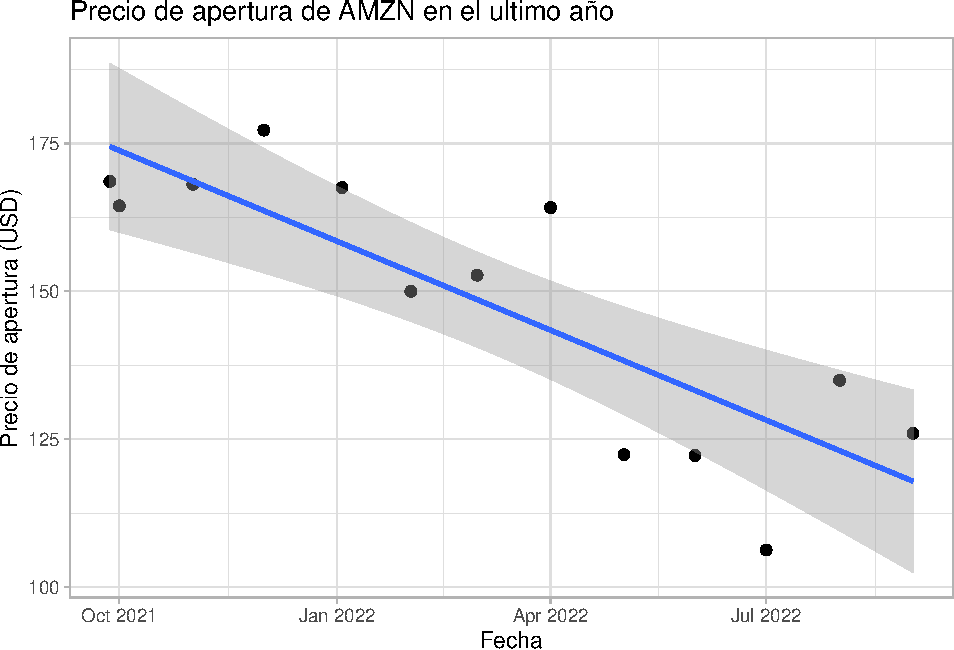
\includegraphics{index_files/figure-latex/unnamed-chunk-3-1.pdf}

\begin{Shaded}
\begin{Highlighting}[]

\NormalTok{sp\_volumen}\OtherTok{\textless{}{-}}\FunctionTok{ggplot}\NormalTok{(data\_precio, }\FunctionTok{aes}\NormalTok{(}\AttributeTok{x=}\NormalTok{ref.date, }\AttributeTok{y=}\NormalTok{volume))}\SpecialCharTok{+}\FunctionTok{geom\_point}\NormalTok{(}\AttributeTok{size =}\DecValTok{2}\NormalTok{, }\AttributeTok{colour =} \StringTok{"black"}\NormalTok{)}\SpecialCharTok{+}\FunctionTok{labs}\NormalTok{(}\AttributeTok{x=}\StringTok{"Fecha"}\NormalTok{, }\AttributeTok{y=}\StringTok{"Volumen"}\NormalTok{, }\AttributeTok{title=}\StringTok{"Volumenes de AMZN en el ultimo año"}\NormalTok{)}\SpecialCharTok{+} \FunctionTok{theme\_light}\NormalTok{()}\SpecialCharTok{+} \FunctionTok{geom\_smooth}\NormalTok{(}\AttributeTok{method =}\NormalTok{ lm, }\AttributeTok{se =} \ConstantTok{TRUE}\NormalTok{)}
\NormalTok{sp\_volumen}
\end{Highlighting}
\end{Shaded}

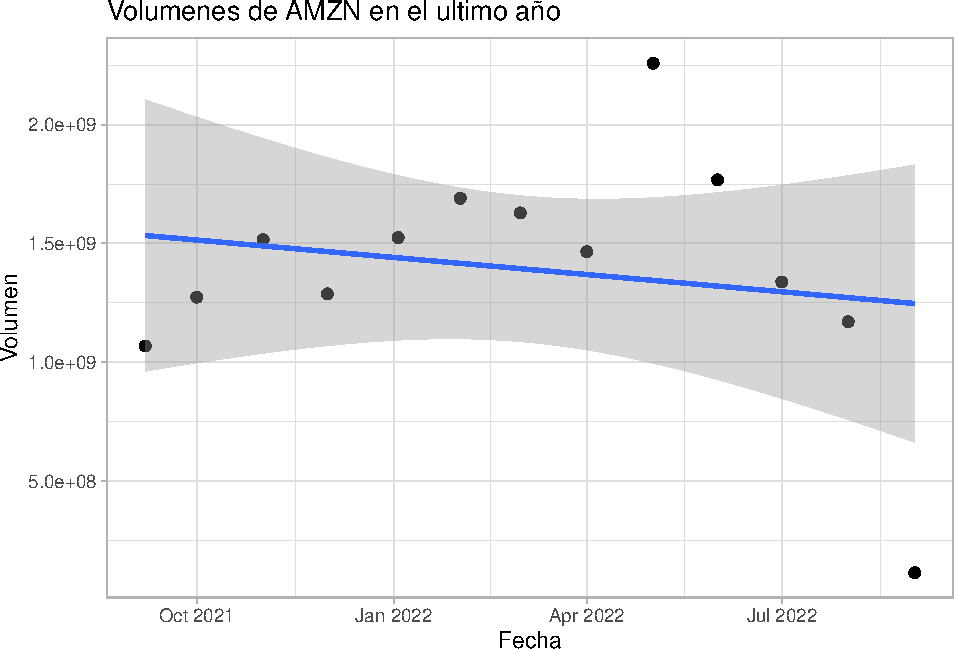
\includegraphics{index_files/figure-latex/unnamed-chunk-3-2.pdf}

\hypertarget{regresiuxf3n-lineal-que-optiene-los-coeficientes-hatboldsymbol-beta}{%
\subsection{\texorpdfstring{Regresión lineal que optiene los coeficientes \(\hat{\boldsymbol \beta}\)}{Regresión lineal que optiene los coeficientes \textbackslash hat\{\textbackslash boldsymbol \textbackslash beta\}}}\label{regresiuxf3n-lineal-que-optiene-los-coeficientes-hatboldsymbol-beta}}

\begin{Shaded}
\begin{Highlighting}[]
\CommentTok{\#datos estadísticos}
\FunctionTok{summary}\NormalTok{(data\_precio[}\FunctionTok{c}\NormalTok{(}\StringTok{"price.open"}\NormalTok{,}\StringTok{"volume"}\NormalTok{)])}
\CommentTok{\#\textgreater{}    price.open        volume         }
\CommentTok{\#\textgreater{}  Min.   :106.3   Min.   :2.694e+08  }
\CommentTok{\#\textgreater{}  1st Qu.:126.0   1st Qu.:1.273e+09  }
\CommentTok{\#\textgreater{}  Median :152.7   Median :1.465e+09  }
\CommentTok{\#\textgreater{}  Mean   :148.1   Mean   :1.397e+09  }
\CommentTok{\#\textgreater{}  3rd Qu.:167.6   3rd Qu.:1.628e+09  }
\CommentTok{\#\textgreater{}  Max.   :177.2   Max.   :2.258e+09}
\CommentTok{\#análisis de regresión lineal lm() y=precio,x=fecha}
\NormalTok{reg\_tiempo\_precio}\OtherTok{\textless{}{-}}\FunctionTok{lm}\NormalTok{(price.open}\SpecialCharTok{\textasciitilde{}}\NormalTok{ref.date, }\AttributeTok{data=}\NormalTok{data\_precio) }
\CommentTok{\#¡Siempre se pone dentro de lm() la variable dependiente primero y luego la independiete!}
\FunctionTok{summary}\NormalTok{(reg\_tiempo\_precio)}
\CommentTok{\#\textgreater{} }
\CommentTok{\#\textgreater{} Call:}
\CommentTok{\#\textgreater{} lm(formula = price.open \textasciitilde{} ref.date, data = data\_precio)}
\CommentTok{\#\textgreater{} }
\CommentTok{\#\textgreater{} Residuals:}
\CommentTok{\#\textgreater{}     Min      1Q  Median      3Q     Max }
\CommentTok{\#\textgreater{} {-}21.955  {-}9.357  {-}0.544   9.431  20.717 }
\CommentTok{\#\textgreater{} }
\CommentTok{\#\textgreater{} Coefficients:}
\CommentTok{\#\textgreater{}               Estimate Std. Error t value Pr(\textgreater{}|t|)    }
\CommentTok{\#\textgreater{} (Intercept) 3328.34629  631.35702   5.272 0.000264 ***}
\CommentTok{\#\textgreater{} ref.date      {-}0.16690    0.03313  {-}5.037 0.000380 ***}
\CommentTok{\#\textgreater{} {-}{-}{-}}
\CommentTok{\#\textgreater{} Signif. codes:  }
\CommentTok{\#\textgreater{} 0 \textquotesingle{}***\textquotesingle{} 0.001 \textquotesingle{}**\textquotesingle{} 0.01 \textquotesingle{}*\textquotesingle{} 0.05 \textquotesingle{}.\textquotesingle{} 0.1 \textquotesingle{} \textquotesingle{} 1}
\CommentTok{\#\textgreater{} }
\CommentTok{\#\textgreater{} Residual standard error: 13.2 on 11 degrees of freedom}
\CommentTok{\#\textgreater{} Multiple R{-}squared:  0.6976, Adjusted R{-}squared:  0.6701 }
\CommentTok{\#\textgreater{} F{-}statistic: 25.37 on 1 and 11 DF,  p{-}value: 0.0003796}

\CommentTok{\#análisis de regresión lineal lm() y=volumen,x=fecha}
\NormalTok{reg\_tiempo\_volumen}\OtherTok{\textless{}{-}}\FunctionTok{lm}\NormalTok{(volume}\SpecialCharTok{\textasciitilde{}}\NormalTok{ref.date, }\AttributeTok{data=}\NormalTok{data\_precio)}
\FunctionTok{summary}\NormalTok{(reg\_tiempo\_volumen)}
\CommentTok{\#\textgreater{} }
\CommentTok{\#\textgreater{} Call:}
\CommentTok{\#\textgreater{} lm(formula = volume \textasciitilde{} ref.date, data = data\_precio)}
\CommentTok{\#\textgreater{} }
\CommentTok{\#\textgreater{} Residuals:}
\CommentTok{\#\textgreater{}        Min         1Q     Median         3Q        Max }
\CommentTok{\#\textgreater{} {-}984384732 {-}167015119   42626028  234203568  807994488 }
\CommentTok{\#\textgreater{} }
\CommentTok{\#\textgreater{} Coefficients:}
\CommentTok{\#\textgreater{}               Estimate Std. Error t value Pr(\textgreater{}|t|)}
\CommentTok{\#\textgreater{} (Intercept) {-}1.588e+10  2.260e+10  {-}0.702    0.497}
\CommentTok{\#\textgreater{} ref.date     9.064e+05  1.186e+06   0.764    0.461}
\CommentTok{\#\textgreater{} }
\CommentTok{\#\textgreater{} Residual standard error: 472300000 on 11 degrees of freedom}
\CommentTok{\#\textgreater{} Multiple R{-}squared:  0.05043,    Adjusted R{-}squared:  {-}0.03589 }
\CommentTok{\#\textgreater{} F{-}statistic: 0.5842 on 1 and 11 DF,  p{-}value: 0.4608}
\end{Highlighting}
\end{Shaded}

\hypertarget{ejercicio}{%
\section{Ejercicio}\label{ejercicio}}

El objetivo de este ejrcicio es simplemente que indiquen y modifiquen los errores en el código. Así pues, deberán descomentar \emph{-quitar las \#antes del código-} para empezar el ejercicio.

\hypertarget{section}{%
\subsection{1}\label{section}}

El objetivo de este código es explicar la variable \textbf{``volume''} con la variable \textbf{``price.high''}.

\begin{Shaded}
\begin{Highlighting}[]
\CommentTok{\#reg\_tiempo\_ej1\textless{}{-}lm(price.high\textasciitilde{}volume, data=data\_precio)}
\CommentTok{\#sumary(reg\_tiempo\_ej1)}
\end{Highlighting}
\end{Shaded}

\hypertarget{section-1}{%
\subsection{2}\label{section-1}}

El objetivo de este código es explicar la variable \textbf{``volume''} con la variable \textbf{``price.low''}.

\begin{Shaded}
\begin{Highlighting}[]
\CommentTok{\#reg\_tiempo\_ej2\textless{}{-}lm(price.low\textasciitilde{}volume, data=data\_precio)}
\CommentTok{\#summary(reg\_tiempo\_ej1)}
\end{Highlighting}
\end{Shaded}

\hypertarget{opcional}{%
\subsection{3 (opcional)}\label{opcional}}

El objetivo de este ejercicio es descargar los valores del stock de Tesla \emph{BMV: TSLA} en los últimos \emph{dos años}.

\begin{Shaded}
\begin{Highlighting}[]
\CommentTok{\#dt\_ej3\textless{}{-}("TSLA")}
\CommentTok{\#pdej\textless{}{-}Sys.Date(){-}(365*3) \#primer fecha}
\CommentTok{\#pdej}
\CommentTok{\#Descargando los valores}
\CommentTok{\#dataej3\textless{}{-} BatchgetSymbols(tickers = dt\_ej3,}
                       \CommentTok{\#first.date = pdej,}
                       \CommentTok{\#last.date = ld,}
                       \CommentTok{\#freq.data = int,}
                       \CommentTok{\#do.cache = FALSE,}
                       \CommentTok{\#thresh.bad.data = 0)}

\CommentTok{\#Generando data frame con los valores}
\CommentTok{\#data\_precio\_ej2\textless{}{-}dataej3$df.tickers}
\CommentTok{\#1colnames(data\_precio\_ej2)}
\end{Highlighting}
\end{Shaded}

\hypertarget{muxe1xima-verosimilitud}{%
\chapter{Máxima Verosimilitud}\label{muxe1xima-verosimilitud}}

\hypertarget{el-problema-1}{%
\section{El problema}\label{el-problema-1}}

Recordemos que dado \(f(y_i | \mathbf{x}_i)\) la función de densidad condicional de \(y_i\) dado \(\mathbf{x}_i\). Sea \(\boldsymbol{\theta}\) un conjunto de parámetros de la función. Entonces la función de densidad conjunta de variables aleatorias independientes \(\{ y_i : y_i \in \mathbb{R} \}\) dados los valores \(\{ \mathbf{x}_i : \mathbf{x}_i \in \mathbb{R}^K \}\) estará dada por:

\begin{equation}
    \Pi_{i = 1}^{n} f(y_i | \mathbf{x}_i; \boldsymbol{\theta}) = f(y_1, y_2, \ldots, y_n | \mathbf{x}_1, \mathbf{x}_2, \ldots, \mathbf{x}_n; \boldsymbol{\theta}) = L(\boldsymbol{\theta})
    \label{eq:EqLikehood}
\end{equation}

A la ecuación \eqref{eq:EqLikehood} se le conoce como ecuación de verosimilitud. El problema de máxima verosimilitud entonces será:
\begin{equation}
    \max_{\boldsymbol{\theta} \in \boldsymbol{\Theta}} \Pi_{i = 1}^{n} f(y_i | \mathbf{x}_i; \boldsymbol{\theta}) = \max_{\boldsymbol{\theta} \in \boldsymbol{\Theta}} L(\boldsymbol{\theta})
        \label{eq:EqMaxLike}
\end{equation}

Dado que el logaritmo natural es una transformación monotona, podemos decir que el problema de la ecuación \eqref{eq:EqMaxLike} es equivalente a:

\begin{equation}
     \max_{\boldsymbol{\theta} \in \boldsymbol{\Theta}} ln L(\boldsymbol{\theta}) = \max_{\boldsymbol{\theta} \in \boldsymbol{\Theta}} ln \Pi_{i = 1}^{n} f(y_i | \mathbf{x}_i; \boldsymbol{\theta}) = \max_{\boldsymbol{\theta} \in \boldsymbol{\Theta}} \sum_{i = 1}^{n} ln f(y_i | \mathbf{x}_i; \boldsymbol{\theta})
            \label{eq:EqLogML}
\end{equation}

Para solucionnar el problema se tiene que determinar las condicones de primer y segundo orden, las cuales serán:
\begin{equation}
    \frac{\partial}{\partial \boldsymbol{\theta}} ln L(\boldsymbol{\theta}) = \nabla ln L(\boldsymbol{\theta})
          \label{eq:MLCPO}
\end{equation}

\begin{equation}
    \frac{\partial^2}{\partial^2 \boldsymbol{\theta}} ln L(\boldsymbol{\theta}) = \frac{\partial}{\partial \boldsymbol{\theta}} ln L(\boldsymbol{\theta}) \cdot  \frac{\partial}{\partial \boldsymbol{\theta}} ln L(\boldsymbol{\theta}') = H(\boldsymbol{\theta})
             \label{eq:MLCSO}
\end{equation}

La solución estará dada por aquel valor de \(\hat{\boldsymbol{\theta}}\) que hace:
\begin{equation*}
    \frac{\partial}{\partial \boldsymbol{\theta}} ln L(\hat{\boldsymbol{\theta}}) = 0
\end{equation*}

A su vez, la varianza será aquella que resulta de:
\begin{equation*}
    Var[\hat{\boldsymbol{\theta}} | \mathbf{X}] = \left( - \mathbb{E}_{\hat{\boldsymbol{\theta}}}[H(\boldsymbol{\theta})] \right)^{-1}
\end{equation*}

\hypertarget{estimaciuxf3n-y-simunlaciuxf3n}{%
\section{Estimación y simunlación}\label{estimaciuxf3n-y-simunlaciuxf3n}}

\hypertarget{lanzar-una-moneda}{%
\subsection{Lanzar una moneda}\label{lanzar-una-moneda}}

\begin{Shaded}
\begin{Highlighting}[]
\FunctionTok{set.seed}\NormalTok{(}\DecValTok{1234}\NormalTok{)}\CommentTok{\#esto sirve para siempre generar los mismos numeros aleatorios}
\CommentTok{\#rbinom(numero observaciones,numero de ensayos,probabilidad de exito en cada ensayo)}
\NormalTok{cara}\OtherTok{\textless{}{-}}\FunctionTok{rbinom}\NormalTok{(}\DecValTok{1}\NormalTok{,}\DecValTok{100}\NormalTok{,}\FloatTok{0.5}\NormalTok{)}
\NormalTok{cara}\CommentTok{\#esto nos dice de los 100 ensayos cuantos fueron cara}
\CommentTok{\#\textgreater{} [1] 47}
\NormalTok{sol}\OtherTok{\textless{}{-}}\DecValTok{100}\SpecialCharTok{{-}}\NormalTok{cara}
\NormalTok{sol}
\CommentTok{\#\textgreater{} [1] 53}


\CommentTok{\#Ahora definiremos la función que encontrará la función de verosimilutud para determinado valor p}
\CommentTok{\#}
\NormalTok{verosimilitud }\OtherTok{\textless{}{-}} \ControlFlowTok{function}\NormalTok{(p)\{}
  \FunctionTok{dbinom}\NormalTok{(cara, }\DecValTok{100}\NormalTok{, p)}
\NormalTok{\}}

\CommentTok{\#si suponemos que la probabilidad sesgada de que caiga cara es 40\%}
\NormalTok{prob\_sesgada}\OtherTok{\textless{}{-}}\FloatTok{0.4}
\CommentTok{\#es posible calcular la función de que salga cara}
\FunctionTok{verosimilitud}\NormalTok{(prob\_sesgada)}
\CommentTok{\#\textgreater{} [1] 0.02919091}
\CommentTok{\#ahora es posible generar una función de verimilitud negativa }
\CommentTok{\#para maximizar el valor de la verosimilitud}
\NormalTok{neg\_verosimilitud }\OtherTok{\textless{}{-}} \ControlFlowTok{function}\NormalTok{(p)\{}
  \FunctionTok{dbinom}\NormalTok{(cara, }\DecValTok{100}\NormalTok{, p)}\SpecialCharTok{*{-}}\DecValTok{1}
\NormalTok{\}}
\FunctionTok{neg\_verosimilitud}\NormalTok{(prob\_sesgada)}
\CommentTok{\#\textgreater{} [1] {-}0.02919091}
\CommentTok{\# unamos la función nlm() para maximizar esta función no linear}
\CommentTok{\#?nlm()}
\FunctionTok{nlm}\NormalTok{(neg\_verosimilitud,}\FloatTok{0.5}\NormalTok{,}\AttributeTok{stepmax=}\FloatTok{0.5}\NormalTok{)}\CommentTok{\#se pone un parametro porque sabemos que hay un 0.5 de probabilidad de que caiga cara}
\CommentTok{\#\textgreater{} $minimum}
\CommentTok{\#\textgreater{} [1] {-}0.07973193}
\CommentTok{\#\textgreater{} }
\CommentTok{\#\textgreater{} $estimate}
\CommentTok{\#\textgreater{} [1] 0.47}
\CommentTok{\#\textgreater{} }
\CommentTok{\#\textgreater{} $gradient}
\CommentTok{\#\textgreater{} [1] 1.589701e{-}10}
\CommentTok{\#\textgreater{} }
\CommentTok{\#\textgreater{} $code}
\CommentTok{\#\textgreater{} [1] 1}
\CommentTok{\#\textgreater{} }
\CommentTok{\#\textgreater{} $iterations}
\CommentTok{\#\textgreater{} [1] 4}
\end{Highlighting}
\end{Shaded}

Si bien el ejercicio anterior es un tanto repetitivo debido a que sabemos que hay un 50\% de que caiga una moneda de un lado o otro. Esto ejemplifica la manera en la que se utiliza el metodo de maximización de máxima verosimilitud.

\hypertarget{muxe9todo-generalizado-de-momentos-mgm}{%
\chapter{Método Generalizado de Momentos (MGM)}\label{muxe9todo-generalizado-de-momentos-mgm}}

\hypertarget{el-problema-2}{%
\section{El problema}\label{el-problema-2}}

Retomemos el modelo de regresión lineal tal que:

\begin{equation}
y_i=X_i\beta+u_i
    \label{Eq_reglin}
\end{equation}

Tomando en cuenta los principios de ortogonalidad (\(E(Z_iu_i)=0\)) y (\(rankE(Z_i^{'}X_i)=0\)) sabemos que \(\beta\) es el único vector de \(N\times1\) que resuelve las condiciones de momento de determinada población. En otras palabras, \(E[z_i^{'}(y_i-x_i\beta)]=0\) es una solución y \(E[z_i^{'}(y_i-x_i\beta)]\neq0\) \emph{NO} es una solución. Debido a que la media muestral son estimadores consistentes de momentos de una población, se puede:

\begin{equation}
N^{-1}\sum_{i=1}^{N}z_i^{'}(y_i-x_i\beta)=0
\label{eq:Eqreglin1asolu1}
\end{equation}

Asumiendo que la ecuación \eqref{eq:Eqreglin1asolu1} tiene L ecuaciones lineales y K coeficientes \(\beta\) desconocidos y \(K=L\), entonces la matriz \(\sum_{i=1}^{N}z_i^{'}x_i\) debe ser no singular para encontrar los coeficientes de la siguiente manera.

\begin{equation}
\hat{\beta}=N^{-1}\left[\sum_{i=1}^{N}z_i^{'}x_i\right]^{-1}\left[\sum_{i=1}^{N}z_i^{'}y_i\right]
\label{eq:Eqreglin1asolu2}
\end{equation}

Para simplificar \eqref{eq:Eqreglin1asolu2} se puede nombrar Z juntando \(z_i\) N veces para crear una matriz de tamaño \(NG\times L\). Lo mismo hacemos con X juntando \(x_i\) para obtener una de \(NG\times K\) y Y obteniendo una \(NG\times 1\). Obteniendo:

\begin{equation}
\hat{\beta}=[Z^{'}X]^{-1}[Z^{'}Y]
\end{equation}

Es importante tomar en cuenta cuando el caso en el que hay más ecuaciones lineales que coeficientes \(\beta\); es decir, \(L\geq K\). En estos casos es muy probrable que no haya solución, por lo que mejor que se puede estimar es pones la ecuación \eqref{eq:Eqreglin1asolu1}, tan pequeña como sea posible. Por lo mismo el paso que nos lleva a la ecuación \eqref{eq:Eqreglin1asolu2}, debe eliminarse \(N^{-1}\). El objetivo:

\begin{equation}
\min_{\beta} \left[\sum_{i=1}^{N}z_i^{'}x_i\beta\right]^{-1}\left[\sum_{i=1}^{N}z_i^{'}y_i\beta\right]
\label{eq:Eqreglin1asolu77}
\end{equation}

Así pues nombramos a W como una matriz simétrica de \(W\times W\) donde se genera la variable \(b\) que debemos minimizar que sustituye a \(\beta\) creando una función cuadrática en la ecuación \eqref{eq:Eqreglin1asolu2}.
\begin{equation}
\min_{b}\left[\sum_{i=1}^{N}z_i^{'}x_ib\right]^{-1}\left[\sum_{i=1}^{N}z_i^{'}y_ib\right]
\label{eq:Eqreglin1asolu78}
\end{equation}

\begin{equation}
\therefore\hat{\beta}=[X^{'}Z\hat{W}Z^{'}X]^{-1}[X^{'}Z\hat{W}Z^{'}Y]
\end{equation}

Sin embargo, \(X^{'}Z\hat{W}Z^{'}X\) debe ser no singular para que haya una solución. Para esto se asume que \(\hat{W}\) tiene un limite de probabilidad no singular. Esto se describe como \(\hat{W}\xrightarrow[]{p}W\) y \(N\xrightarrow[]{}W\infty\) donde \(W\) no es aleatorio, es una matriz positiva definida simétrica de \(L\times L\).

\hypertarget{capital-asset-pricing-model-capm}{%
\chapter{CAPITAL ASSET PRICING MODEL (CAPM)}\label{capital-asset-pricing-model-capm}}

\hypertarget{el-problema-3}{%
\section{El problema}\label{el-problema-3}}

Una vez que hemos establecido la manera en la que se pueden estimar algunos valores --como las regresiones lineales y el método de máxima verosimilitud--, además de la naturaleza de los retornos de algunos activos en el capítulo 4, es posible comenzar a hablar de maneras en la que se pueden estimar los valores futuros de los rendimientos de activos y --de esta manera-- poder tomar mejores decisiones de inversiones. Por ello, hablaremos del modelo de \textbf{Capital Asset Pricing Model}. El modelo es muy sencillo y pretende estimar su rentabilidad esperada en función del \textbf{riesgo sistemático}. Por lo mismo, en este modelo se utilizan los valores de los precios de los activos a lo largo del tiempo y utiliza la intuición con la que derivamos la ecuación lineal con los Mínimos cuadrados ordinarios (MCO).

\begin{equation}
    R_{jt}-R{ft}=\alpha_{j}+\beta_j(R_{mt}-R_{ft})+u_{jt}
\label{eq:CAMP}
\end{equation}

En la ecuación \eqref{eq:CAMP}

\begin{itemize}
\item
  \(R_{jt}\) es el retorno del portafolio \(j\) en el tiempo \(t\)
\item
  \(R_{ft}\) es el retorno de un bono sin riesgo gubernamental en un año. \textbf{Parecido a los CETES}.
\item
  \(R_{mt}\) es el retorno en un portafolio de mercado.
\item
  \(u_{jt}\) es el retorno en un portafolio de mercado.
\item
  \(\alpha_{j},\beta_j\) son los coeficientes que queremos obtener.
\end{itemize}

De esta manera, \(\alpha_j\) es el coeficiente que más nos interesa debido a que queremos ver si el activo supera o no el index del mercado con base en el activo fijo.

Si \(\alpha_j\) es positivo entonces sabemos que el retorno tiene buenos rendimiendtos y uno negativo significa que no. Por tanto \(H_0:\alpha_j=0\)

\hypertarget{estimaciuxf3n-r-1}{%
\section{Estimación R}\label{estimaciuxf3n-r-1}}

Para la estimación utilizaremos el paquete ``BatchGetSymbols''. Este paquete nos permitirá descargar información acerca de la bolsa de valores internacional.

\hypertarget{estimaciuxf3n}{%
\section{ESTIMACIÓN}\label{estimaciuxf3n}}

\hypertarget{dependencias-1}{%
\subsection{Dependencias}\label{dependencias-1}}

\begin{Shaded}
\begin{Highlighting}[]
\CommentTok{\#install.packages("pacman")}
\CommentTok{\#pacman nos permite cargar varias librerias en una sola línea}
\FunctionTok{library}\NormalTok{(pacman)}
\NormalTok{pacman}\SpecialCharTok{::}\FunctionTok{p\_load}\NormalTok{(tidyverse,BatchGetSymbols,ggplot2,lubridate,readxl,tidyquant)}
\end{Highlighting}
\end{Shaded}

\hypertarget{descarga-de-los-valores-1}{%
\subsection{Descarga de los valores}\label{descarga-de-los-valores-1}}

\begin{Shaded}
\begin{Highlighting}[]
\CommentTok{\#Primero determinamos el lapso de tiempo}
\NormalTok{pd}\OtherTok{\textless{}{-}}\FunctionTok{as.Date}\NormalTok{(}\StringTok{"2021/09/18"}\NormalTok{) }\CommentTok{\#primer fecha}
\NormalTok{pd}
\CommentTok{\#\textgreater{} [1] "2021{-}09{-}18"}
\NormalTok{ld}\OtherTok{\textless{}{-}}\FunctionTok{as.Date}\NormalTok{(}\StringTok{"2022/09/18"}\NormalTok{) }\CommentTok{\#última fecha}
\NormalTok{ld}
\CommentTok{\#\textgreater{} [1] "2022{-}09{-}18"}
\CommentTok{\#Intervalos de tiempo}
\NormalTok{int}\OtherTok{\textless{}{-}}\StringTok{"monthly"}
\CommentTok{\#Datos a elegir}
\NormalTok{dt}\OtherTok{\textless{}{-}}\FunctionTok{c}\NormalTok{(}\StringTok{"AMZN"}\NormalTok{)}
\NormalTok{dt2}\OtherTok{\textless{}{-}}\FunctionTok{c}\NormalTok{(}\StringTok{"TSLA"}\NormalTok{)}
\CommentTok{\#Descargando los valores}
\NormalTok{?}\FunctionTok{BatchGetSymbols}\NormalTok{()}
\NormalTok{data1}\OtherTok{\textless{}{-}} \FunctionTok{BatchGetSymbols}\NormalTok{(}\AttributeTok{tickers =}\NormalTok{ dt,}
                       \AttributeTok{first.date =}\NormalTok{ pd,}
                       \AttributeTok{last.date =}\NormalTok{ ld,}
                       \AttributeTok{freq.data =}\NormalTok{ int,}
                       \AttributeTok{do.cache =} \ConstantTok{FALSE}\NormalTok{,}
                       \AttributeTok{thresh.bad.data =} \DecValTok{0}\NormalTok{)}
\NormalTok{data2}\OtherTok{\textless{}{-}} \FunctionTok{BatchGetSymbols}\NormalTok{(}\AttributeTok{tickers =}\NormalTok{ dt2,}
                       \AttributeTok{first.date =}\NormalTok{ pd,}
                       \AttributeTok{last.date =}\NormalTok{ ld,}
                       \AttributeTok{freq.data =}\NormalTok{ int,}
                       \AttributeTok{do.cache =} \ConstantTok{FALSE}\NormalTok{,}
                       \AttributeTok{thresh.bad.data =} \DecValTok{0}\NormalTok{)}

\CommentTok{\#Generando data frame con los valores}
\NormalTok{data\_precio\_amzn}\OtherTok{\textless{}{-}}\NormalTok{data1}\SpecialCharTok{$}\NormalTok{df.tickers}
\FunctionTok{colnames}\NormalTok{(data\_precio\_amzn)}
\CommentTok{\#\textgreater{}  [1] "ticker"              "ref.date"           }
\CommentTok{\#\textgreater{}  [3] "volume"              "price.open"         }
\CommentTok{\#\textgreater{}  [5] "price.high"          "price.low"          }
\CommentTok{\#\textgreater{}  [7] "price.close"         "price.adjusted"     }
\CommentTok{\#\textgreater{}  [9] "ret.adjusted.prices" "ret.closing.prices"}
\NormalTok{data\_precio\_tls}\OtherTok{\textless{}{-}}\NormalTok{data2}\SpecialCharTok{$}\NormalTok{df.tickers}
\FunctionTok{colnames}\NormalTok{(data\_precio\_tls)}
\CommentTok{\#\textgreater{}  [1] "ticker"              "ref.date"           }
\CommentTok{\#\textgreater{}  [3] "volume"              "price.open"         }
\CommentTok{\#\textgreater{}  [5] "price.high"          "price.low"          }
\CommentTok{\#\textgreater{}  [7] "price.close"         "price.adjusted"     }
\CommentTok{\#\textgreater{}  [9] "ret.adjusted.prices" "ret.closing.prices"}
\CommentTok{\#necesitamos convertir la serie de tiempo de precios en retornos continuos compuestos de los precios de apertura}
\NormalTok{data\_precio\_amzn}\SpecialCharTok{$}\NormalTok{ccrAMZN}\OtherTok{\textless{}{-}}\FunctionTok{c}\NormalTok{(}\ConstantTok{NA}\NormalTok{ ,}\DecValTok{100}\SpecialCharTok{*}\FunctionTok{diff}\NormalTok{(}\FunctionTok{log}\NormalTok{(data\_precio\_amzn}\SpecialCharTok{$}\NormalTok{price.open)))}\CommentTok{\#agregamos un valor NA al principio}
\NormalTok{data\_precio\_amzn}\SpecialCharTok{$}\NormalTok{ccrAMZN}\CommentTok{\#estos son los retornos}
\CommentTok{\#\textgreater{}  [1]          NA  {-}3.2011678   2.1889913   5.3061639}
\CommentTok{\#\textgreater{}  [5]  {-}5.6279333 {-}11.0646538   1.8052718   7.2089622}
\CommentTok{\#\textgreater{}  [9] {-}29.3475086  {-}0.1185366 {-}13.9945965  23.8807273}
\CommentTok{\#\textgreater{} [13]  {-}6.8696583}

\NormalTok{data\_precio\_tls}\SpecialCharTok{$}\NormalTok{ccrTSLA}\OtherTok{\textless{}{-}}\FunctionTok{c}\NormalTok{(}\ConstantTok{NA}\NormalTok{ ,}\DecValTok{100}\SpecialCharTok{*}\FunctionTok{diff}\NormalTok{(}\FunctionTok{log}\NormalTok{(data\_precio\_tls}\SpecialCharTok{$}\NormalTok{price.open)))}\CommentTok{\#agregamos un valor NA al principio}
\NormalTok{data\_precio\_tls}\SpecialCharTok{$}\NormalTok{ccrTSLA}
\CommentTok{\#\textgreater{}  [1]         NA   5.796888  38.591933   1.361865  {-}1.121972}
\CommentTok{\#\textgreater{}  [6] {-}20.478772  {-}7.264574  21.765521 {-}22.795320 {-}13.089771}
\CommentTok{\#\textgreater{} [11] {-}10.336735  28.307900 {-}10.009692}
\CommentTok{\#formateando por año y mes}
\NormalTok{data\_precio\_tls}\SpecialCharTok{$}\NormalTok{ref.date}\OtherTok{=}\FunctionTok{format}\NormalTok{(}\FunctionTok{as.Date}\NormalTok{(data\_precio\_tls}\SpecialCharTok{$}\NormalTok{ref.date), }\StringTok{"\%m/\%Y"}\NormalTok{)}
\NormalTok{data\_precio\_amzn}\SpecialCharTok{$}\NormalTok{ref.date}\OtherTok{=}\FunctionTok{format}\NormalTok{(}\FunctionTok{as.Date}\NormalTok{(data\_precio\_amzn}\SpecialCharTok{$}\NormalTok{ref.date), }\StringTok{"\%m/\%Y"}\NormalTok{)}
\CommentTok{\#Compararemos con los CETES}
\NormalTok{CETES\_sep2021\_2022}\OtherTok{\textless{}{-}}\FunctionTok{read\_excel}\NormalTok{(}\StringTok{"BD/CETES{-}sep2021{-}2022.xlsx"}\NormalTok{, }\AttributeTok{skip=}\DecValTok{17}\NormalTok{)}
\FunctionTok{head}\NormalTok{(CETES\_sep2021\_2022)}
\CommentTok{\#\textgreater{} \# A tibble: 6 x 2}
\CommentTok{\#\textgreater{}   Fecha               SF43936}
\CommentTok{\#\textgreater{}   \textless{}dttm\textgreater{}                \textless{}dbl\textgreater{}}
\CommentTok{\#\textgreater{} 1 2021{-}09{-}15 00:00:00    4.6 }
\CommentTok{\#\textgreater{} 2 2021{-}09{-}23 00:00:00    4.58}
\CommentTok{\#\textgreater{} 3 2021{-}09{-}30 00:00:00    4.69}
\CommentTok{\#\textgreater{} 4 2021{-}10{-}07 00:00:00    4.81}
\CommentTok{\#\textgreater{} 5 2021{-}10{-}14 00:00:00    4.79}
\CommentTok{\#\textgreater{} 6 2021{-}10{-}21 00:00:00    4.83}
\CommentTok{\#indice sp500}
\NormalTok{SP500 }\OtherTok{\textless{}{-}} \FunctionTok{read\_csv}\NormalTok{(}\StringTok{"BD/Download Data {-} INDEX\_US\_S\&P US\_SPX.csv"}\NormalTok{)}
\NormalTok{SP500}\SpecialCharTok{$}\NormalTok{ccrSP500}\OtherTok{\textless{}{-}}\FunctionTok{c}\NormalTok{(}\ConstantTok{NA}\NormalTok{ ,}\DecValTok{100}\SpecialCharTok{*}\FunctionTok{diff}\NormalTok{(}\FunctionTok{log}\NormalTok{(SP500}\SpecialCharTok{$}\NormalTok{Open)))}
\FunctionTok{names}\NormalTok{(SP500)[}\DecValTok{1}\NormalTok{]}\OtherTok{\textless{}{-}}\FunctionTok{paste}\NormalTok{(}\StringTok{\textquotesingle{}ref.date\textquotesingle{}}\NormalTok{)}
\CommentTok{\#formateando por año y mes}

\CommentTok{\#cetes}
\NormalTok{cete\_1\_año}\OtherTok{\textless{}{-}}\FloatTok{10.10}\CommentTok{\#esto es el rendimiento a un año de un cete gubernamental seguro}

\CommentTok{\#Juntamos el df}
\NormalTok{CAPM\_2}\OtherTok{\textless{}{-}}\FunctionTok{merge}\NormalTok{(data\_precio\_amzn, data\_precio\_tls, }\AttributeTok{by =} \FunctionTok{c}\NormalTok{(}\StringTok{\textquotesingle{}ref.date\textquotesingle{}}\NormalTok{))}
\NormalTok{CAPM\_4}\OtherTok{\textless{}{-}}\FunctionTok{merge}\NormalTok{(SP500, CAPM\_2, }\AttributeTok{by =} \FunctionTok{c}\NormalTok{(}\StringTok{\textquotesingle{}ref.date\textquotesingle{}}\NormalTok{))}
\NormalTok{CAPM}\OtherTok{\textless{}{-}}\FunctionTok{data.frame}\NormalTok{(CAPM\_4)}

\CommentTok{\#exceso de retorno}
\NormalTok{CAPM}\SpecialCharTok{$}\NormalTok{excess\_ret\_AMZN}\OtherTok{\textless{}{-}}\NormalTok{CAPM}\SpecialCharTok{$}\NormalTok{ccrAMZN}\SpecialCharTok{{-}}\NormalTok{cete\_1\_año}
\NormalTok{CAPM}\SpecialCharTok{$}\NormalTok{excess\_ret\_SP500}\OtherTok{\textless{}{-}}\NormalTok{CAPM}\SpecialCharTok{$}\NormalTok{ccrSP500}\SpecialCharTok{{-}}\NormalTok{cete\_1\_año}
\NormalTok{CAPM}\SpecialCharTok{$}\NormalTok{excess\_ret\_TSLA}\OtherTok{\textless{}{-}}\NormalTok{CAPM}\SpecialCharTok{$}\NormalTok{ccrTSLA}\SpecialCharTok{{-}}\NormalTok{cete\_1\_año}
\end{Highlighting}
\end{Shaded}

\begin{Shaded}
\begin{Highlighting}[]
\CommentTok{\#relacion entre los excesos de demanda}
\FunctionTok{ggplot}\NormalTok{(CAPM, }\FunctionTok{aes}\NormalTok{(}\AttributeTok{x=}\NormalTok{excess\_ret\_AMZN, }\AttributeTok{y=}\NormalTok{excess\_ret\_SP500))}\SpecialCharTok{+}\FunctionTok{geom\_point}\NormalTok{()}\SpecialCharTok{+}\FunctionTok{labs}\NormalTok{(}\AttributeTok{title=}\StringTok{"Relación de excesos de retornos entre TSLA y AMZN"}\NormalTok{,}\AttributeTok{y=}\StringTok{"Exceso de demanda de SP500"}\NormalTok{, }\AttributeTok{x=}\StringTok{"Exceso de demanda de AMZN"}\NormalTok{)}\SpecialCharTok{+}\FunctionTok{theme\_light}\NormalTok{()}
\CommentTok{\#\textgreater{} Warning: Removed 2 rows containing missing values}
\CommentTok{\#\textgreater{} (geom\_point).}
\end{Highlighting}
\end{Shaded}

\begin{figure}
\centering
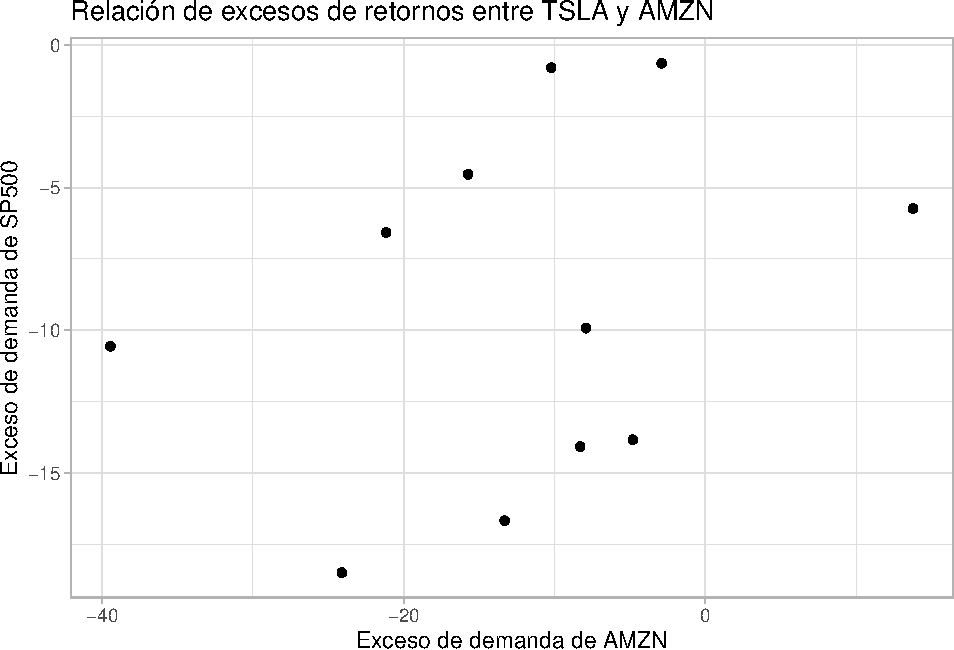
\includegraphics{04-CAPM_files/figure-latex/TSTSLAAMAZN1-1.pdf}
\caption{\label{fig:TSTSLAAMAZN1}Relación de excesos de retornos entre AMZN y SP500}
\end{figure}

\begin{Shaded}
\begin{Highlighting}[]
\CommentTok{\#relacion entre los excesos de demanda}
\FunctionTok{ggplot}\NormalTok{(CAPM, }\FunctionTok{aes}\NormalTok{(}\AttributeTok{x=}\NormalTok{excess\_ret\_TSLA, }\AttributeTok{y=}\NormalTok{excess\_ret\_SP500))}\SpecialCharTok{+}\FunctionTok{geom\_point}\NormalTok{()}\SpecialCharTok{+}\FunctionTok{labs}\NormalTok{(}\AttributeTok{title=}\StringTok{"Relación de excesos de retornos entre TSLA y AMZN"}\NormalTok{,}\AttributeTok{y=}\StringTok{"Exceso de demanda de SP500"}\NormalTok{, }\AttributeTok{x=}\StringTok{"Exceso de demanda de TSLA"}\NormalTok{)}\SpecialCharTok{+}\FunctionTok{theme\_light}\NormalTok{()}
\CommentTok{\#\textgreater{} Warning: Removed 2 rows containing missing values}
\CommentTok{\#\textgreater{} (geom\_point).}
\end{Highlighting}
\end{Shaded}

\begin{figure}
\centering
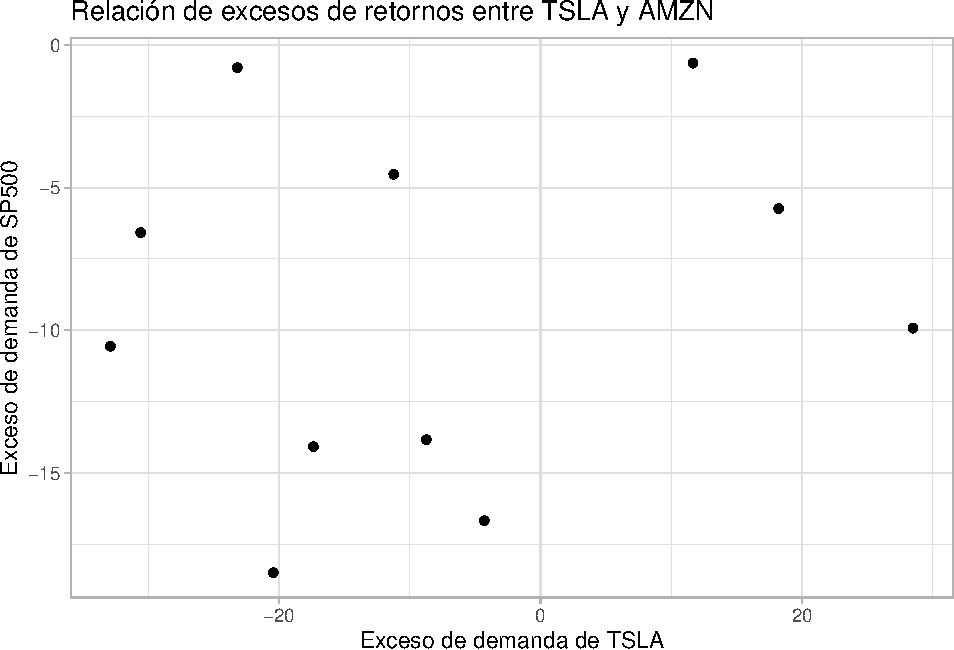
\includegraphics{04-CAPM_files/figure-latex/TSTSLAAMAZN2-1.pdf}
\caption{\label{fig:TSTSLAAMAZN2}Relación de excesos de retornos entre TSLA y SP500}
\end{figure}

\begin{Shaded}
\begin{Highlighting}[]
\CommentTok{\#veamos la regresion lineal}
\NormalTok{CAPM\_lr}\OtherTok{\textless{}{-}}\FunctionTok{lm}\NormalTok{(excess\_ret\_TSLA}\SpecialCharTok{\textasciitilde{}}\NormalTok{excess\_ret\_SP500,}\AttributeTok{data =}\NormalTok{ CAPM)}
\FunctionTok{summary}\NormalTok{(CAPM\_lr)}
\CommentTok{\#\textgreater{} }
\CommentTok{\#\textgreater{} Call:}
\CommentTok{\#\textgreater{} lm(formula = excess\_ret\_TSLA \textasciitilde{} excess\_ret\_SP500, data = CAPM)}
\CommentTok{\#\textgreater{} }
\CommentTok{\#\textgreater{} Residuals:}
\CommentTok{\#\textgreater{}     Min      1Q  Median      3Q     Max }
\CommentTok{\#\textgreater{} {-}23.980 {-}13.391  {-}5.548  11.572  37.067 }
\CommentTok{\#\textgreater{} }
\CommentTok{\#\textgreater{} Coefficients:}
\CommentTok{\#\textgreater{}                  Estimate Std. Error t value Pr(\textgreater{}|t|)}
\CommentTok{\#\textgreater{} (Intercept)       {-}3.2334    11.8097  {-}0.274     0.79}
\CommentTok{\#\textgreater{} excess\_ret\_SP500   0.5379     1.0789   0.499     0.63}
\CommentTok{\#\textgreater{} }
\CommentTok{\#\textgreater{} Residual standard error: 20.88 on 9 degrees of freedom}
\CommentTok{\#\textgreater{}   (2 observations deleted due to missingness)}
\CommentTok{\#\textgreater{} Multiple R{-}squared:  0.02687,    Adjusted R{-}squared:  {-}0.08125 }
\CommentTok{\#\textgreater{} F{-}statistic: 0.2486 on 1 and 9 DF,  p{-}value: 0.6301}
\NormalTok{alpha1}\OtherTok{\textless{}{-}}\FunctionTok{coefficients}\NormalTok{(CAPM\_lr)[}\DecValTok{1}\NormalTok{]}
\NormalTok{alpha1}\SpecialCharTok{\textless{}}\DecValTok{0}
\CommentTok{\#\textgreater{} (Intercept) }
\CommentTok{\#\textgreater{}        TRUE}
\end{Highlighting}
\end{Shaded}

De esta manera sabemos que el rendimiento de TSLA NO es mayor debido a que el coeficiente \(\alpha=-2.9534\), lo cual indica peores rendimientos al resto del SP500.

\hypertarget{ejercicio-compara-con-tsla-con-el-apple}{%
\section{Ejercicio Compara con TSLA con el APPLE}\label{ejercicio-compara-con-tsla-con-el-apple}}

\begin{Shaded}
\begin{Highlighting}[]
\NormalTok{dt3}\OtherTok{\textless{}{-}}\StringTok{"AAPL"}
\NormalTok{data3}\OtherTok{\textless{}{-}}\FunctionTok{BatchGetSymbols}\NormalTok{(}\AttributeTok{tickers =}\NormalTok{ dt3,}
                       \AttributeTok{first.date =}\NormalTok{ pd,}
                       \AttributeTok{last.date =}\NormalTok{ ld,}
                       \AttributeTok{freq.data =}\NormalTok{ int,}
                       \AttributeTok{do.cache =} \ConstantTok{FALSE}\NormalTok{,}
                       \AttributeTok{thresh.bad.data =} \DecValTok{0}\NormalTok{)}
\CommentTok{\#\textgreater{} Warning: \textasciigrave{}BatchGetSymbols()\textasciigrave{} was deprecated in BatchGetSymbols 2.6.4.}
\CommentTok{\#\textgreater{} Please use \textasciigrave{}yfR::yf\_get()\textasciigrave{} instead.}
\CommentTok{\#\textgreater{} 2022{-}05{-}01: Package BatchGetSymbols will soon be replaced by yfR. }
\CommentTok{\#\textgreater{} More details about the change is available at github \textless{}\textless{}www.github.com/msperlin/yfR\textgreater{}}
\CommentTok{\#\textgreater{} You can install yfR by executing:}
\CommentTok{\#\textgreater{} }
\CommentTok{\#\textgreater{} remotes::install\_github(\textquotesingle{}msperlin/yfR\textquotesingle{})}
\CommentTok{\#\textgreater{} }
\CommentTok{\#\textgreater{} Running BatchGetSymbols for:}
\CommentTok{\#\textgreater{}    tickers =AAPL}
\CommentTok{\#\textgreater{}    Downloading data for benchmark ticker}
\CommentTok{\#\textgreater{} \^{}GSPC | yahoo (1|1)}
\CommentTok{\#\textgreater{} AAPL | yahoo (1|1) {-} Got 100\% of valid prices | Looking good!}
\NormalTok{data\_precio\_AAPL}\OtherTok{\textless{}{-}}\NormalTok{data3}\SpecialCharTok{$}\NormalTok{df.tickers}
\FunctionTok{colnames}\NormalTok{(data\_precio\_AAPL)}
\CommentTok{\#\textgreater{}  [1] "ticker"              "ref.date"           }
\CommentTok{\#\textgreater{}  [3] "volume"              "price.open"         }
\CommentTok{\#\textgreater{}  [5] "price.high"          "price.low"          }
\CommentTok{\#\textgreater{}  [7] "price.close"         "price.adjusted"     }
\CommentTok{\#\textgreater{}  [9] "ret.adjusted.prices" "ret.closing.prices"}
\NormalTok{data\_precio\_AAPL}\SpecialCharTok{$}\NormalTok{ccrAAPL}\OtherTok{\textless{}{-}}\FunctionTok{c}\NormalTok{(}\ConstantTok{NA}\NormalTok{ ,}\DecValTok{100}\SpecialCharTok{*}\FunctionTok{diff}\NormalTok{(}\FunctionTok{log}\NormalTok{(data\_precio\_AAPL}\SpecialCharTok{$}\NormalTok{price.open)))}\CommentTok{\#agregamos un valor NA al principio}
\NormalTok{data\_precio\_AAPL}\SpecialCharTok{$}\NormalTok{ccrAAPL}
\CommentTok{\#\textgreater{}  [1]         NA  {-}1.330092   4.875668  11.698469   5.996413}
\CommentTok{\#\textgreater{}  [6]  {-}2.171531  {-}5.498712   5.510207 {-}10.483068  {-}4.442864}
\CommentTok{\#\textgreater{} [11]  {-}9.701946  16.851754  {-}2.751627}
\NormalTok{data\_precio\_AAPL}\SpecialCharTok{$}\NormalTok{ref.date}\OtherTok{=}\FunctionTok{format}\NormalTok{(}\FunctionTok{as.Date}\NormalTok{(data\_precio\_AAPL}\SpecialCharTok{$}\NormalTok{ref.date), }\StringTok{"\%m/\%Y"}\NormalTok{)}
\NormalTok{CAPM\_3}\OtherTok{\textless{}{-}}\FunctionTok{merge}\NormalTok{(data\_precio\_AAPL, CAPM, }\AttributeTok{by =} \FunctionTok{c}\NormalTok{(}\StringTok{\textquotesingle{}ref.date\textquotesingle{}}\NormalTok{))}
\NormalTok{CAPM\_3}\SpecialCharTok{$}\NormalTok{excess\_ret\_AAPL}\OtherTok{\textless{}{-}}\NormalTok{CAPM\_3}\SpecialCharTok{$}\NormalTok{ccrAAPL}\SpecialCharTok{{-}}\NormalTok{cete\_1\_año}
\CommentTok{\#veamos la regresion lineal}
\NormalTok{CAPM3\_lr}\OtherTok{\textless{}{-}}\FunctionTok{lm}\NormalTok{(excess\_ret\_AAPL}\SpecialCharTok{\textasciitilde{}}\NormalTok{excess\_ret\_SP500,}\AttributeTok{data =}\NormalTok{ CAPM\_3)}
\FunctionTok{summary}\NormalTok{(CAPM3\_lr)}
\CommentTok{\#\textgreater{} }
\CommentTok{\#\textgreater{} Call:}
\CommentTok{\#\textgreater{} lm(formula = excess\_ret\_AAPL \textasciitilde{} excess\_ret\_SP500, data = CAPM\_3)}
\CommentTok{\#\textgreater{} }
\CommentTok{\#\textgreater{} Residuals:}
\CommentTok{\#\textgreater{}      Min       1Q   Median       3Q      Max }
\CommentTok{\#\textgreater{} {-}10.9038  {-}5.4365   0.4641   3.4629  14.1798 }
\CommentTok{\#\textgreater{} }
\CommentTok{\#\textgreater{} Coefficients:}
\CommentTok{\#\textgreater{}                  Estimate Std. Error t value Pr(\textgreater{}|t|)}
\CommentTok{\#\textgreater{} (Intercept)       {-}4.7542     4.9105  {-}0.968    0.358}
\CommentTok{\#\textgreater{} excess\_ret\_SP500   0.4663     0.4486   1.039    0.326}
\CommentTok{\#\textgreater{} }
\CommentTok{\#\textgreater{} Residual standard error: 8.682 on 9 degrees of freedom}
\CommentTok{\#\textgreater{}   (2 observations deleted due to missingness)}
\CommentTok{\#\textgreater{} Multiple R{-}squared:  0.1072, Adjusted R{-}squared:  0.007964 }
\CommentTok{\#\textgreater{} F{-}statistic:  1.08 on 1 and 9 DF,  p{-}value: 0.3258}
\NormalTok{alpha2}\OtherTok{\textless{}{-}}\FunctionTok{coefficients}\NormalTok{(CAPM3\_lr)[}\DecValTok{1}\NormalTok{]}
\NormalTok{alpha2}\SpecialCharTok{\textless{}}\DecValTok{0}
\CommentTok{\#\textgreater{} (Intercept) }
\CommentTok{\#\textgreater{}        TRUE}
\end{Highlighting}
\end{Shaded}

\hypertarget{estacionariedad}{%
\chapter{Estacionariedad}\label{estacionariedad}}

\hypertarget{el-problema-4}{%
\section{El problema}\label{el-problema-4}}

Los fundamentos de las series de tiempo están basados en la
estacionalidad. Una serie de tiempo \({r_t}\) que estudia los retornos de
un activo a lo largo de tiempo es \emph{estrictamente estacionaria} si la
distribución conjunta de los retornos \((r_{t1},\dots,r_{t1})\) es
\emph{exactamente idéntica} en \((r_{t1+T},\dots,r_{t1+T})\), es decir cuando
pasa \(T\) años, por ejemplo. En otras palabras, definiremos a una serie
de tiempo como un vector de variables \({X_t}\) aleatorias de dimensión
\(T\), dado como:

\begin{equation}
    X_1, X_2, X_3, \ldots ,X_T
\end{equation}

Es decir, definiremos a una serie de tiempo como una
realización de un proceso estocástico --o un Proceso Generador de Datos
(PGD). Consideremos una muestra de los múltiples posibles resultados de
muestras de tamaño \(T\), la colección dada por:

\begin{equation}
    \{X^{(1)}_1, X^{(1)}_2, \ldots, X^{(1)}_T\}
    \label{eq:variast}
\end{equation}

Eventualmente podríamos estar dispuestos a observar este proceso
indefinidamente, de forma tal que estemos interesados en observar a la
secuencia dada por \(\{ X^{(1)}_t \}^{\infty}_{t = 1}\), lo cual no
dejaría se ser sólo una de las tantas realizaciones o secuencias del
proceso estocástico original de la ecuación \eqref{eq:variast}.

\begin{eqnarray*}
    & \{X^{(2)}_1, X^{(2)}_2, \ldots, X^{(2)}_T\} & \\
    & \{X^{(3)}_1, X^{(3)}_2, \ldots, X^{(3)}_T\} & \\
    & \{X^{(4)}_1, X^{(4)}_2, \ldots, X^{(4)}_T\} & \\
    & \vdots & \\
    & \{X^{(j)}_1, X^{(j)}_2, \ldots, X^{(j)}_T\} & 
\end{eqnarray*}

Por lo mismo, cada cambio que se hace al vector \(\{ X^{(1)}_t \}\) es
parte del mismo proceso estocástico, por lo que la serie de tiempo es:

\begin{equation}
    \{ X_1, X_2, \ldots, X_T \}
        \label{variast}
\end{equation}

El proceso estocástico de dimensión \(T\) puede ser completamente descrito
por su función de distribución multivariada de dimensión \(T\). No
obstante, sólo nos enfocaremos en sus primer y segundo momentos, es
decir, en sus medias o valores esperados \(\mathbb{E} (X_t)\)

Para \(t = 1, 2, \ldots, T\):

\begin{equation*}
\left[
    \begin{array}{c}
    \mathbb{E}[X_1], \mathbb{E}[X_2], \ldots, \mathbb{E}[X_T]
    \end{array}
\right]
\end{equation*}

De sus variazas:

\begin{equation*}
    Var[X_t] = \mathbb{E}[(X_t - \mathbb{E}[X_t])^2]
\end{equation*} Para \(t = 1, 2, \ldots, T\), y de sus \(T(T-1)/2\)
covarianzas: \begin{equation*}
    Cov[X_t,X_s] = \mathbb{E}[(X_t - \mathbb{E}[X_t])(X_s - \mathbb{E}[X_s])]
\end{equation*}

Para \(t < s\). Por lo tanto, en la forma matricial podemos escribir lo siguiente:
\begin{equation*}
\left[
    \begin{array}{c c c c}
    Var[X_1] & Cov[X_1,X_2] & \cdots & Cov[X_1,X_T] \\
    Cov[X_2,X_1] & Var[X_2] & \cdots & Cov[X_2,X_T] \\
    \vdots & \vdots & \ddots & \vdots \\
    Cov[X_T,X_1] & Cov[X_T,X_2] & \cdots & Var[X_T] \\
    \end{array}
\right]
\end{equation*}

\begin{equation}
= \left[
    \begin{array}{c c c c}
    \sigma_1^2 & \rho_{12} & \cdots & \rho_{1T} \\
    \rho_{21} & \sigma_2^2 & \cdots & \rho_{2T} \\
    \vdots & \vdots & \ddots & \vdots \\
    \rho_{T1} & \rho_{T2} & \cdots & \sigma_T^2 \\
    \end{array}
\right]
\label{eq:MATCOV}
\end{equation}

Donde es claro que en la matriz de la ecuación \eqref{eq:MATCOV} existen \(T(T-1)/2\) covarianzas distintas, ya que se cumple que \(Cov[X_t,X_s] = Cov[X_s,X_t]\), para \(t \neq s\). A menudo, esas covarianzas son denominadas como \emph{autocovarianzas} puesto que ellas son covarianzas entre variables aleatorias pertenecientes al mismo proceso estocástico pero en un momento \(t\) diferente. Si el proceso estocástico tiene una distribución normal multivariada, su función de distribución estará totalmente descrita por sus momentos de primer y segundo orden.

\hypertarget{ergocidad}{%
\subsection{Ergocidad}\label{ergocidad}}

Esto implica que los momentos muestrales, los cuales son calculados en la base de una serie de tiempo con un número finito de observaciones, conforme el tiempo \(T \rightarrow \infty\) sus correspondientes momentos muestrales, tienden a los verdaderos valores poblacionales, los cuales definiremos como \(\mu\), para la media, y \(\sigma^2_X\) para la varianza. \emph{En pocas palabras, conforme los momentos muestrales aumenten tanto que tiendan al infinito, entonces nos acercamos a valores poblacionales de la media y la varianza}.
Este concepto sólo es cierto si asumimos que

\begin{eqnarray*}
    \mathbb{E}[X_t] = \mu_t = \mu \\
    Var[X_t] = \sigma^2_X
\end{eqnarray*}
Más formalmente, se dice que el PGD o el proceso estocástico es ergódico en la media si:
\begin{equation}
    \displaystyle\lim_{T \to \infty}{\mathbb{E} \left[ \left( \frac{1}{T} \sum^{T}_{t = 1} (X_t - \mu) \right) ^2 \right]} = 0
\end{equation}

y ergódico en la varianza si:
\begin{equation}
    \displaystyle\lim_{T \to \infty}{\mathbb{E} \left[ \left( \frac{1}{T} \sum^{T}_{t = 1} (X_t - \mu) ^2 - \sigma^2_X \right) ^2 \right]} = 0
\end{equation}
+
Estas condiciones se les conoce como \emph{propiedades de consistencia} para las variables aleatorias. Sin embargo, éstas no pueden ser probadas. Por ello se les denomina como un supuesto que pueden cumplir algunas de las series. Más importante aún: \textbf{un proceso estocástico que tiende a estar en equilibrio estadístico en un orden ergódico, es estacionario}.

\hypertarget{tipos-de-estacionariedad}{%
\subsection{Tipos de Estacionariedad}\label{tipos-de-estacionariedad}}

Definiremos a la estacionariedad por sus momentos del correspondiente proceso estocástico dado por \(\{X_t\}\):

\begin{itemize}
\item
  \emph{Estacionariedad en media}: Un proceso estocástico es estacionario en media si \(E[X_t] = \mu_t = \mu\) es constante para todo \(t\).
\item
  \emph{Estacionariedad en varianza}: Un proceso estocástico es estacionario en varianza si \(Var[X_t] = \mathbb{E}[(X_t - \mu_t)^2] = \sigma^2_X = \gamma(0)\) es constante y finita para todo \(t\).
\item
  \emph{Estacionariedad en covarianza}: Un proceso estocástico es estacionario en covarianza si \(Cov[X_t,X_s] = \mathbb{E}[(X_t - \mu_t)(X_s - \mu_s)] = \gamma(|s-t|)\) es sólo una función del tiempo y de la distancia entre las dos variables aleatorias. Por lo que no depende del tiempo denotado por \(t\) (no depende de la información contemporánea).
\item
  \emph{Estacionariedad débil}: Como la estacionariedad en varianza resulta de forma inmediata de la estacionariedad en covarianza cuando se asume que \(s = t\), un proceso estocástico es débilmente estacionario cuando es estacionario en media y covarianza. \textbf{ESTE ES EL MÁS COMÚN Y POSIBLE}, por lo que es el que estudiaremos.
\end{itemize}

\hypertarget{funciuxf3n-de-autocorrelaciuxf3n-acf}{%
\subsection{Función de Autocorrelación (ACF)}\label{funciuxf3n-de-autocorrelaciuxf3n-acf}}

Para ampliar la discusión, es posible calcular la fuerza o intensidad de la dependencia de las variables aleatorias dentro de un proceso estocástico, ello mediante el uso de las autocovarianzas. Cuando las covarianzas son normalizadas respecto de la varianza, el resultado es un término que es independiente de las unidad de medida aplicada, y se conoce como la \emph{función de autocorrelación}.

Por su parte, un estimador consistente de la función de autocorrelación estará dado por:
\begin{equation}
    \hat{\rho}(\tau) = \frac{\sum^{T - \tau}_{t=1} (X_t - \hat{\mu})(X_{t+\tau} - \hat{\mu})}{\sum^T_{t=1} (X_t - \hat{\mu})^2} = \frac{\hat{\gamma}(\tau)}{\hat{\gamma}(0)} \mbox{, para } \tau = 1, 2, \ldots, T-1
    \label{eq:EqAutoCorr}
\end{equation}

El estimador de la ecuación \eqref{eq:EqAutoCorr} es asintóticamente insesgado y \textbf{es relevante puesto que nos dice si una serie de tiempo con estacionariedad débil esta serialmente correlacionada si y solo si \(\hat{\rho}(\tau)\neq0\)}.

\hypertarget{ruido-blanco}{%
\subsection{Ruido Blanco}\label{ruido-blanco}}

Supongamos una serie de tiempo denotada por: \(\{U_t\}^T_{t = 0}\). Decimos que el proceso estocástico \(\{U_t\}\) es un \emph{proceso estocástico puramente aleatorio} o es un \emph{proceso estocástico de ruido blanco o caminata aleatoria}, si éste tiene las siguientes propiedades:

\begin{itemize}
\item
  \(\mathbb{E}[U_t] = 0\), \(\forall t\)
\item
  \(Var[U_t] = \mathbb{E}[(U_t - \mu_t)^2] = \mathbb{E}[(U_t - \mu)^2] = \mathbb{E}[(U_t)^2] = \sigma^2\), \(\forall t\)
\item
  \(Cov[U_t,U_s] = \mathbb{E}[(U_t - \mu_t)(U_s - \mu_s)] = \mathbb{E}[(U_t - \mu)(U_s - \mu)] = \mathbb{E}[U_t U_s] = 0\), \(\forall t \neq s\).
\item
  \(\hat{\rho}(\tau)=0\)
\end{itemize}

En palabras. Un proceso \(U_t\) es un ruido blanco si su valor promedio es cero (0), tiene una varianza finita y constante, y además no le importa la historia pasada, así su valor presente no se ve influenciado por sus valores pasados no importando respecto de que periodo se tome referencia.

Para procesos estacionarios, dicha función de autocorrelación esta dada por:
\begin{equation}
    \rho(\tau) = \frac{\mathbb{E}[(X_t - \mu)(X_{t+\tau} - \mu)]}{\mathbb{E}[(X_t - \mu)^2]} = \frac{\gamma(\tau)}{\gamma(0)} 
\end{equation}

\hypertarget{estimaciuxf3n-1}{%
\section{Estimación}\label{estimaciuxf3n-1}}

\hypertarget{dependencias-2}{%
\subsection{Dependencias}\label{dependencias-2}}

\begin{Shaded}
\begin{Highlighting}[]
\CommentTok{\#install.packages("pacman")}
\CommentTok{\#pacman nos permite cargar varias librerias en una sola línea}
\FunctionTok{library}\NormalTok{(pacman)}
\NormalTok{pacman}\SpecialCharTok{::}\FunctionTok{p\_load}\NormalTok{(tidyverse,BatchGetSymbols,ggplot2,lubridate,readxl,forecast,stats)}
\end{Highlighting}
\end{Shaded}

\hypertarget{caminata}{%
\section{Caminata}\label{caminata}}

\begin{Shaded}
\begin{Highlighting}[]

\FunctionTok{set.seed}\NormalTok{(}\DecValTok{1234}\NormalTok{)}
\CommentTok{\# Utilizaremos una función guardada en un archivo a parte}
\CommentTok{\# Llamamos a la función:}
\FunctionTok{source}\NormalTok{(}\StringTok{"funciones/Caminata.R"}\NormalTok{)}

\CommentTok{\# Definimos argumentos de la función}
\NormalTok{Opciones }\OtherTok{\textless{}{-}} \FunctionTok{c}\NormalTok{(}\SpecialCharTok{{-}}\DecValTok{1}\NormalTok{, }\DecValTok{1}\NormalTok{)}
\CommentTok{\#}
\NormalTok{Soporte }\OtherTok{\textless{}{-}} \DecValTok{10000}

\CommentTok{\# Vamos a réplicar el proceso con estos parámetros}
\NormalTok{Rango }\OtherTok{\textless{}{-}} \DecValTok{200}
\CommentTok{\#}
\NormalTok{Caminos }\OtherTok{\textless{}{-}} \DecValTok{10}

\CommentTok{\#}

\ControlFlowTok{for}\NormalTok{(i }\ControlFlowTok{in} \DecValTok{1}\SpecialCharTok{:}\NormalTok{Caminos)\{}
\NormalTok{  TT }\OtherTok{\textless{}{-}} \FunctionTok{data.matrix}\NormalTok{(}\FunctionTok{data.frame}\NormalTok{(}\FunctionTok{Caminata}\NormalTok{(Opciones, Soporte)[}\DecValTok{1}\NormalTok{]))}
  \CommentTok{\#}
\NormalTok{  G\_t }\OtherTok{\textless{}{-}} \FunctionTok{data.matrix}\NormalTok{(}\FunctionTok{data.frame}\NormalTok{(}\FunctionTok{Caminata}\NormalTok{(Opciones, Soporte)[}\DecValTok{2}\NormalTok{]))}
  \CommentTok{\#}
  \FunctionTok{plot}\NormalTok{(TT, G\_t, }\AttributeTok{col =} \StringTok{"blue"}\NormalTok{, }\AttributeTok{type =} \StringTok{"l"}\NormalTok{, }\AttributeTok{ylab =} \StringTok{"Ganancias"}\NormalTok{, }\AttributeTok{xlab =} \StringTok{"Tiempo"}\NormalTok{, }\AttributeTok{ylim =} \FunctionTok{c}\NormalTok{(}\SpecialCharTok{{-}}\NormalTok{Rango,Rango))}
  \CommentTok{\#}
  \FunctionTok{par}\NormalTok{(}\AttributeTok{new =} \ConstantTok{TRUE}\NormalTok{)}
  \CommentTok{\#}
\NormalTok{  i }\OtherTok{\textless{}{-}}\NormalTok{ i }\SpecialCharTok{+}\DecValTok{1}
\NormalTok{\}}
\CommentTok{\#}
\FunctionTok{par}\NormalTok{(}\AttributeTok{new =} \ConstantTok{FALSE}\NormalTok{)}
\end{Highlighting}
\end{Shaded}

\begin{figure}

{\centering 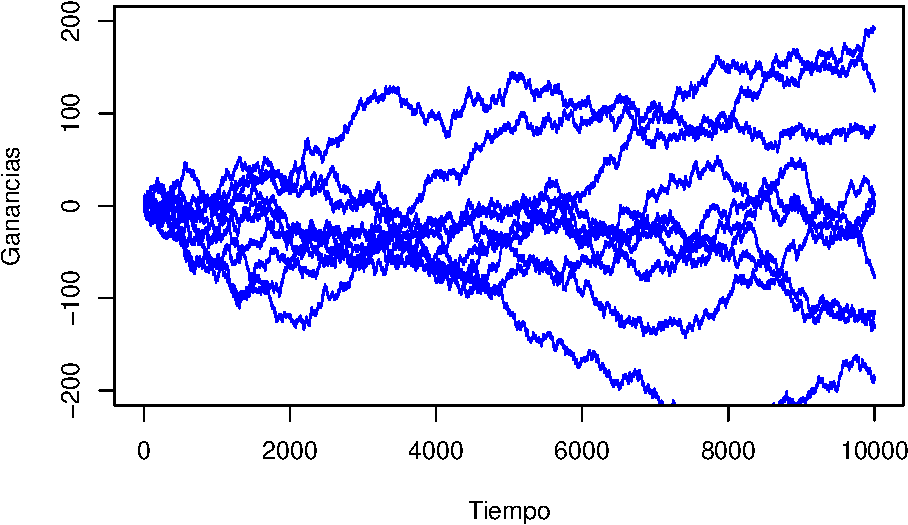
\includegraphics{06-ESTACIONARIEDAD_files/figure-latex/Caminata10-1} 

}

\caption{Ejemplo de 10 trayectorias de la caminata aleatoria, cuando sólo es posible cambios de +1 y -1}\label{fig:Caminata10}
\end{figure}

Así, el proceso estocástico dado por la caminata alaeatoria sin un
término de ajuste es estacionario en media, pero no en varianza o en
covarianza, y consecuentemente, en general no estacionario, condición
que contraria al caso del proceso simple descrito en \(U_t\).

Es facil ver que muchas de las posibilidades de realización de este
proceso estocástico (series de tiempo) pueden tomar cualquiera de las
rutas consideradas en el Figura \ref{fig:Caminata10}. Ahora analicemos
un solo camino.

\hypertarget{un-camino}{%
\section{Un camino}\label{un-camino}}

\begin{Shaded}
\begin{Highlighting}[]
\CommentTok{\#Generamos datos}
\NormalTok{  TT1 }\OtherTok{\textless{}{-}} \FunctionTok{data.matrix}\NormalTok{(}\FunctionTok{data.frame}\NormalTok{(}\FunctionTok{Caminata}\NormalTok{(Opciones, Soporte)[}\DecValTok{1}\NormalTok{]))}
\NormalTok{  G\_t1 }\OtherTok{\textless{}{-}} \FunctionTok{data.matrix}\NormalTok{(}\FunctionTok{data.frame}\NormalTok{(}\FunctionTok{Caminata}\NormalTok{(Opciones, Soporte)[}\DecValTok{2}\NormalTok{]))}
\CommentTok{\#Creemos un data frame}
\NormalTok{  dt\_caminata}\OtherTok{\textless{}{-}}\FunctionTok{data.frame}\NormalTok{(TT1,G\_t1)}
  \FunctionTok{colnames}\NormalTok{(dt\_caminata)}\OtherTok{\textless{}{-}}\FunctionTok{c}\NormalTok{(}\StringTok{"t"}\NormalTok{,}\StringTok{"ganancias"}\NormalTok{)}
  \FunctionTok{head}\NormalTok{(dt\_caminata)}
\CommentTok{\#\textgreater{}   t ganancias}
\CommentTok{\#\textgreater{} 1 1        {-}1}
\CommentTok{\#\textgreater{} 2 2        {-}2}
\CommentTok{\#\textgreater{} 3 3        {-}1}
\CommentTok{\#\textgreater{} 4 4        {-}2}
\CommentTok{\#\textgreater{} 5 5        {-}3}
\CommentTok{\#\textgreater{} 6 6        {-}4}
\CommentTok{\#plot}
  \FunctionTok{plot}\NormalTok{(TT1, G\_t1, }\AttributeTok{col =} \StringTok{"blue"}\NormalTok{, }\AttributeTok{type =} \StringTok{"l"}\NormalTok{, }\AttributeTok{ylab =} \StringTok{"Ganancias"}\NormalTok{, }\AttributeTok{xlab =} \StringTok{"Tiempo"}\NormalTok{, }\AttributeTok{ylim =} \FunctionTok{c}\NormalTok{(}\SpecialCharTok{{-}}\NormalTok{Rango,Rango))}
\end{Highlighting}
\end{Shaded}

\begin{figure}
\centering
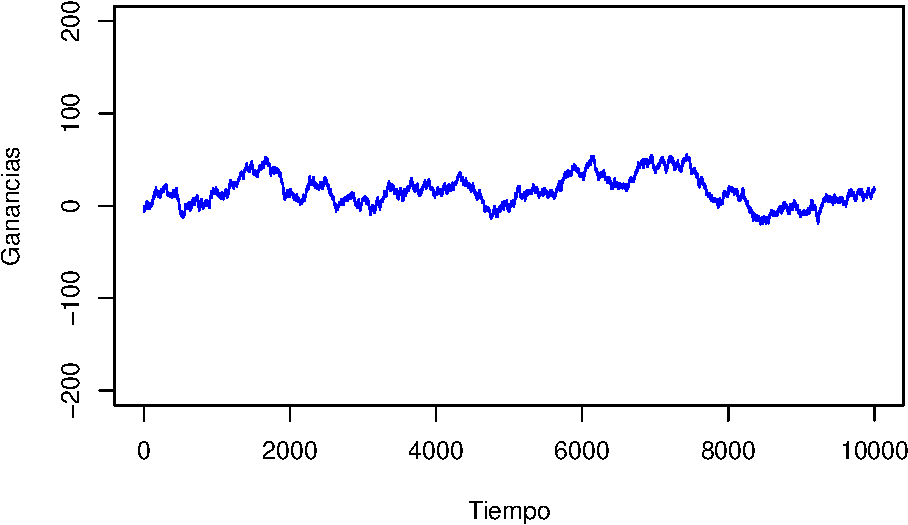
\includegraphics{06-ESTACIONARIEDAD_files/figure-latex/Caminata1-1.pdf}
\caption{\label{fig:Caminata1}Una Caminata aleatoria cuando sólo es posible cambios de +1 y -1}
\end{figure}

Hay que convertirlo a serie de tiempo

\begin{Shaded}
\begin{Highlighting}[]
\CommentTok{\#serie de tiempo}
\NormalTok{caminata\_ts}\OtherTok{\textless{}{-}}\FunctionTok{ts}\NormalTok{(G\_t1,}\AttributeTok{start=}\DecValTok{1}\NormalTok{,}\AttributeTok{end=}\NormalTok{Soporte)}
\end{Highlighting}
\end{Shaded}

\hypertarget{estacionariedad-caminata}{%
\subsection{Estacionariedad Caminata}\label{estacionariedad-caminata}}

\begin{Shaded}
\begin{Highlighting}[]
\NormalTok{ACF\_caminata\_ts}\OtherTok{\textless{}{-}}\FunctionTok{acf}\NormalTok{(caminata\_ts,}\AttributeTok{na.action =}\NormalTok{ na.pass, }\AttributeTok{main =} \StringTok{"Función de Autocorrelación de una Caminata"}\NormalTok{)}
\end{Highlighting}
\end{Shaded}

\begin{figure}
\centering
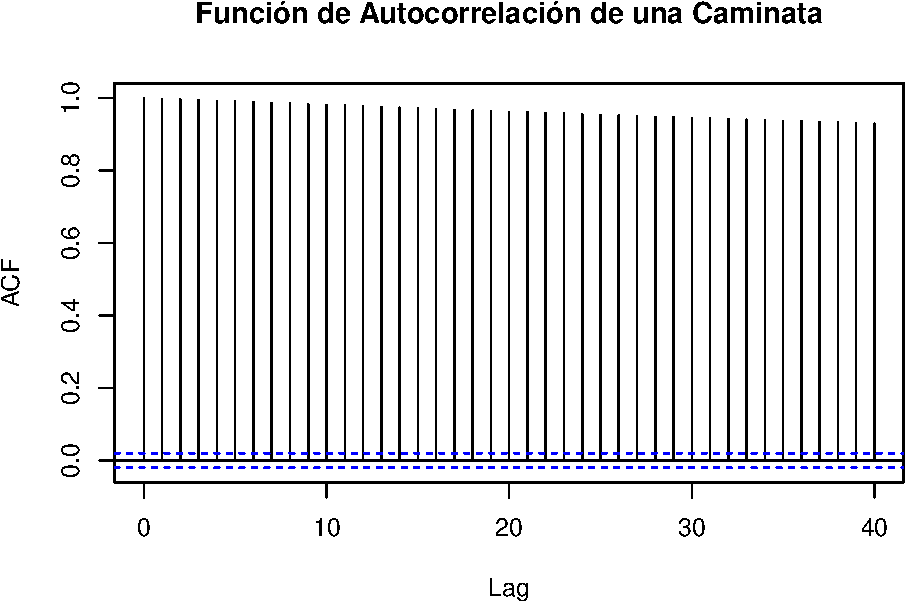
\includegraphics{06-ESTACIONARIEDAD_files/figure-latex/ACFCAMINATA1-1.pdf}
\caption{\label{fig:ACFCAMINATA1}Función de Autocorrelación de una Caminata}
\end{figure}

Como se comentó con anterioridad en la Figura \ref{fig:ACFCAMINATA1} es
evidente que la Caminata si tiene autocorrelacion, por lo que nuestro
plot de autocorrelacion tiene valores muy altos en todos los lags.
Veamos los lags.

\begin{Shaded}
\begin{Highlighting}[]
\FunctionTok{gglagplot}\NormalTok{(caminata\_ts,}\AttributeTok{lags=}\DecValTok{10}\NormalTok{,}\AttributeTok{do.lines=}\ConstantTok{FALSE}\NormalTok{,}\AttributeTok{colour=}\ConstantTok{FALSE}\NormalTok{)}\SpecialCharTok{+}\FunctionTok{theme\_light}\NormalTok{()}
\end{Highlighting}
\end{Shaded}

\begin{figure}
\centering
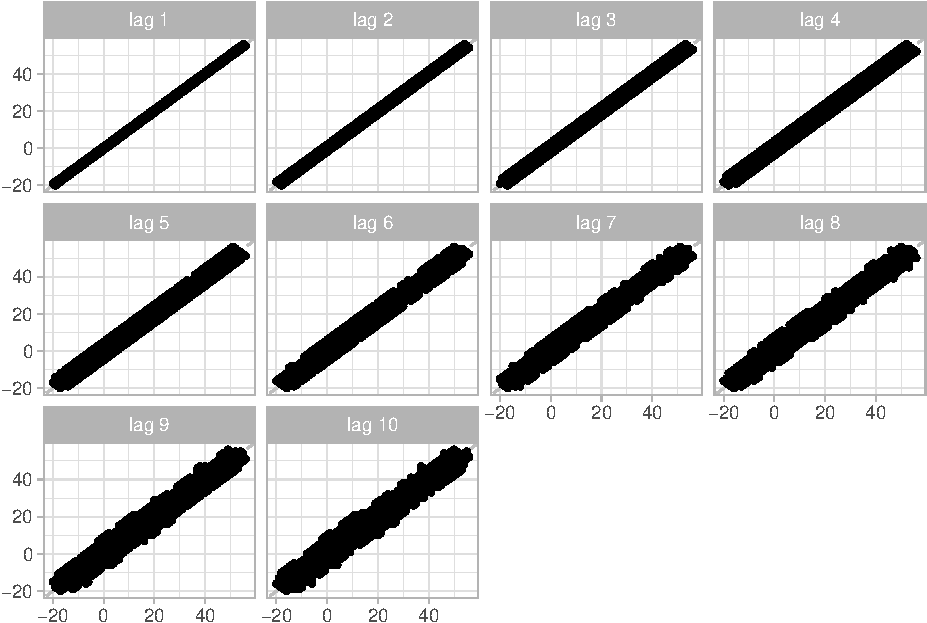
\includegraphics{06-ESTACIONARIEDAD_files/figure-latex/LAGSCAMINATA1-1.pdf}
\caption{\label{fig:LAGSCAMINATA1}Lags de una sola caminata}
\end{figure}

De nuevo, esto al ser creado de manera estandarizada estamos seguros de
que va a ser estacionario en la medio, por lo mismo los lags de la
Figura \ref{fig:LAGSCAMINATA1} se ven tan correlacionados.

\hypertarget{precios-de-un-activo}{%
\section{Precios de un activo}\label{precios-de-un-activo}}

\begin{Shaded}
\begin{Highlighting}[]
\CommentTok{\#Primero determinamos el lapso de tiempo}
\NormalTok{pd}\OtherTok{\textless{}{-}}\FunctionTok{Sys.Date}\NormalTok{()}\SpecialCharTok{{-}}\NormalTok{(}\DecValTok{365}\SpecialCharTok{*}\DecValTok{20}\NormalTok{) }\CommentTok{\#primer fecha}
\NormalTok{pd}
\CommentTok{\#\textgreater{} [1] "2002{-}10{-}02"}
\NormalTok{ld}\OtherTok{\textless{}{-}}\FunctionTok{Sys.Date}\NormalTok{() }\CommentTok{\#última fecha}
\NormalTok{ld}
\CommentTok{\#\textgreater{} [1] "2022{-}09{-}27"}
\CommentTok{\#Intervalos de tiempo}
\NormalTok{int}\OtherTok{\textless{}{-}}\StringTok{"monthly"}
\CommentTok{\#Datos a elegir}
\NormalTok{dt}\OtherTok{\textless{}{-}}\FunctionTok{c}\NormalTok{(}\StringTok{"AMZN"}\NormalTok{)}
\NormalTok{dt2}\OtherTok{\textless{}{-}}\FunctionTok{c}\NormalTok{(}\StringTok{"TSLA"}\NormalTok{)}
\CommentTok{\#Descargando los valores}
\NormalTok{data1}\OtherTok{\textless{}{-}} \FunctionTok{BatchGetSymbols}\NormalTok{(}\AttributeTok{tickers =}\NormalTok{ dt,}
                       \AttributeTok{first.date =}\NormalTok{ pd,}
                       \AttributeTok{last.date =}\NormalTok{ ld,}
                       \AttributeTok{freq.data =}\NormalTok{ int,}
                       \AttributeTok{do.cache =} \ConstantTok{FALSE}\NormalTok{,}
                       \AttributeTok{thresh.bad.data =} \DecValTok{0}\NormalTok{)}
\CommentTok{\#Generando data frame con los valores}
\NormalTok{data\_precio\_amzn}\OtherTok{\textless{}{-}}\NormalTok{data1}\SpecialCharTok{$}\NormalTok{df.tickers}
\FunctionTok{colnames}\NormalTok{(data\_precio\_amzn)}
\CommentTok{\#\textgreater{}  [1] "ticker"              "ref.date"           }
\CommentTok{\#\textgreater{}  [3] "volume"              "price.open"         }
\CommentTok{\#\textgreater{}  [5] "price.high"          "price.low"          }
\CommentTok{\#\textgreater{}  [7] "price.close"         "price.adjusted"     }
\CommentTok{\#\textgreater{}  [9] "ret.adjusted.prices" "ret.closing.prices"}

\CommentTok{\#necesitamos convertir la serie de tiempo de precios en retornos continuos compuestos de los precios de apertura}
\NormalTok{data\_precio\_amzn}\SpecialCharTok{$}\NormalTok{ccrAMZN}\OtherTok{\textless{}{-}}\FunctionTok{c}\NormalTok{(}\ConstantTok{NA}\NormalTok{ ,}\DecValTok{100}\SpecialCharTok{*}\FunctionTok{diff}\NormalTok{(}\FunctionTok{log}\NormalTok{(data\_precio\_amzn}\SpecialCharTok{$}\NormalTok{price.open)))}\CommentTok{\#agregamos un valor NA al principio}
\NormalTok{data\_precio\_amzn}\SpecialCharTok{$}\NormalTok{ccrAMZN}\CommentTok{\#estos son los retornos}
\CommentTok{\#\textgreater{}   [1]           NA  13.39774561  22.83329766 {-}22.98950701}
\CommentTok{\#\textgreater{}   [5]  13.39221448   0.95260416  14.27998202  11.55626991}
\CommentTok{\#\textgreater{}   [9]  24.11122449  {-}0.46684144  13.08785513  11.63599301}
\CommentTok{\#\textgreater{}  [13]   3.89974592  12.48104071  {-}0.73260401  {-}3.06108260}
\CommentTok{\#\textgreater{}  [17]  {-}4.08140972 {-}16.32741069   0.99457279   0.06902105}
\CommentTok{\#\textgreater{}  [21]   9.61879412  11.67844638 {-}33.59147712  {-}0.57381482}
\CommentTok{\#\textgreater{}  [25]   7.69997922 {-}18.78100714  15.60691856  11.66713068}
\CommentTok{\#\textgreater{}  [29]  {-}4.43506452 {-}20.41392362  {-}1.23405211  {-}6.96531282}
\CommentTok{\#\textgreater{}  [33]   9.64353557  {-}6.77486160  30.02382912  {-}5.40177077}
\CommentTok{\#\textgreater{}  [37]   6.39945115 {-}12.58398922  20.12391421  {-}2.92703823}
\CommentTok{\#\textgreater{}  [41]  {-}7.77281354 {-}15.93630872  {-}2.10477279  {-}4.11970307}
\CommentTok{\#\textgreater{}  [45]  {-}1.60415929  10.64572285 {-}37.21478392  15.01070027}
\CommentTok{\#\textgreater{}  [49]   3.59739571  17.58906665   5.43570463  {-}4.00357496}
\CommentTok{\#\textgreater{}  [53]  {-}1.90531667   3.54637914   1.33891100  42.77167396}
\CommentTok{\#\textgreater{}  [57]  11.98170332  {-}0.13070948  12.66409736   2.27857959}
\CommentTok{\#\textgreater{}  [61]  15.63296023  {-}6.26135927   2.56510858   5.74113839}
\CommentTok{\#\textgreater{}  [65] {-}18.78533471 {-}21.72447597  13.78662202   7.15014819}
\CommentTok{\#\textgreater{}  [69]   3.44753666 {-}11.63053849   5.54650897   8.53074641}
\CommentTok{\#\textgreater{}  [73] {-}14.71605773 {-}24.20236452 {-}29.39126222  20.09953181}
\CommentTok{\#\textgreater{}  [77]  13.15576837   8.77225235  13.27882326   9.60320128}
\CommentTok{\#\textgreater{}  [81]  {-}2.73678724   7.64068237   2.50334747  {-}6.96036997}
\CommentTok{\#\textgreater{}  [85]  13.59745291  24.90536163  14.32806129  {-}0.50514401}
\CommentTok{\#\textgreater{}  [89] {-}10.08447333  {-}3.70473986  13.45839135   1.02565002}
\CommentTok{\#\textgreater{}  [93]  {-}9.33660068 {-}13.76436786   8.99531736   5.87517724}
\CommentTok{\#\textgreater{}  [97]  21.76202538   4.58513429   8.56726887   1.22598823}
\CommentTok{\#\textgreater{} [101]  {-}6.16865517   1.74979032   4.53458328   7.93222740}
\CommentTok{\#\textgreater{} [105]  {-}0.25978671   4.72685785   9.04110889  {-}4.41608958}
\CommentTok{\#\textgreater{} [109]   0.80039290  {-}4.18766494  {-}8.13529694  {-}8.68550170}
\CommentTok{\#\textgreater{} [113]  {-}1.18960511   3.43828044   9.60224827  14.70991690}
\CommentTok{\#\textgreater{} [117]  {-}9.58159747   9.53799598   2.08880372   5.85976366}
\CommentTok{\#\textgreater{} [121]   2.83140800  {-}8.65274050   7.52661134   1.39202437}
\CommentTok{\#\textgreater{} [125]   4.89612270  {-}2.12710012   1.39936277  {-}5.02332605}
\CommentTok{\#\textgreater{} [129]   5.76221809   3.66491122   8.27850152  {-}6.24554343}
\CommentTok{\#\textgreater{} [133]   9.85520147  15.15285156   8.73395739  {-}0.05013788}
\CommentTok{\#\textgreater{} [137] {-}10.51934673  {-}0.06687288  {-}5.92858190 {-}10.58568315}
\CommentTok{\#\textgreater{} [141]   2.74371861   4.15753522  {-}3.80625428   8.04816141}
\CommentTok{\#\textgreater{} [145]  {-}5.42111518  {-}5.03065911   9.90317538  {-}7.85404256}
\CommentTok{\#\textgreater{} [149]  11.32156221   8.43295383  {-}2.32429615  13.01462014}
\CommentTok{\#\textgreater{} [153]   1.54061721   2.05813986  20.15392877  {-}7.39490376}
\CommentTok{\#\textgreater{} [157]   2.34828935  20.47843365   7.17052347  {-}2.62563883}
\CommentTok{\#\textgreater{} [161] {-}12.67694180  {-}3.85435390   5.96629237  11.72089295}
\CommentTok{\#\textgreater{} [165]   8.23387458  {-}0.49783030   5.76252931   1.44112456}
\CommentTok{\#\textgreater{} [169]   8.10699776  {-}4.52676184  {-}6.00796092   0.72964776}
\CommentTok{\#\textgreater{} [173]   8.98955770   2.83447462   4.01536256   4.38443827}
\CommentTok{\#\textgreater{} [177]   7.35281333  {-}2.61760725   2.36894617  {-}1.20285851}
\CommentTok{\#\textgreater{} [181]  {-}2.07377928  13.68712240   5.85471090  {-}0.00427124}
\CommentTok{\#\textgreater{} [185]  20.93976645   4.63815978  {-}6.55115525   9.77684681}
\CommentTok{\#\textgreater{} [189]   4.61358018   2.75160333   5.84583306  12.74521370}
\CommentTok{\#\textgreater{} [193]  {-}0.22279328 {-}21.94794383   8.60716489 {-}18.86826361}
\CommentTok{\#\textgreater{} [197]  11.20213025   0.98664739   8.39682297   7.12720047}
\CommentTok{\#\textgreater{} [201]  {-}9.38002536   8.85565506  {-}2.70183034  {-}5.58782369}
\CommentTok{\#\textgreater{} [205]  {-}1.36520548   2.37757442   0.91249016   3.83805218}
\CommentTok{\#\textgreater{} [209]   6.98245156  {-}5.31693095   1.37938043  18.97247680}
\CommentTok{\#\textgreater{} [213]   4.64889431  11.92308161  14.25393454   9.27398656}
\CommentTok{\#\textgreater{} [217]  {-}8.41337555  {-}4.66642316   4.05671846   2.52393793}
\CommentTok{\#\textgreater{} [221]  {-}0.84885499  {-}3.59427728  {-}0.31861156  11.12179968}
\CommentTok{\#\textgreater{} [225]  {-}7.17375312   5.72503641  {-}2.40180912   4.18486227}
\CommentTok{\#\textgreater{} [229]  {-}6.11473001   2.18899134   5.30616390  {-}5.62793333}
\CommentTok{\#\textgreater{} [233] {-}11.06465380   1.80527180   7.20896224 {-}29.34750864}
\CommentTok{\#\textgreater{} [237]  {-}0.11853658 {-}13.99459654  23.88072732  {-}6.86965832}
\CommentTok{\#tenemos 20 retornos a lo largo de 20 años}
\end{Highlighting}
\end{Shaded}

Veamos la serie de tiempo

\begin{Shaded}
\begin{Highlighting}[]
\NormalTok{ret\_20\_amazn}\OtherTok{\textless{}{-}}\FunctionTok{ggplot}\NormalTok{(}\AttributeTok{data=}\NormalTok{data\_precio\_amzn, }\FunctionTok{aes}\NormalTok{(}\AttributeTok{x=}\NormalTok{ref.date))}\SpecialCharTok{+}\FunctionTok{geom\_line}\NormalTok{(}\FunctionTok{aes}\NormalTok{(}\AttributeTok{y=}\NormalTok{ccrAMZN))}\SpecialCharTok{+}\FunctionTok{labs}\NormalTok{(}\AttributeTok{title=}\StringTok{"Retornos de AMZN en los últimos 20 años"}\NormalTok{,}\AttributeTok{y=}\StringTok{"Retornos"}\NormalTok{, }\AttributeTok{x=}\StringTok{"Años"}\NormalTok{)}\SpecialCharTok{+}\FunctionTok{theme\_light}\NormalTok{()}
\NormalTok{ret\_20\_amazn}
\end{Highlighting}
\end{Shaded}

\begin{figure}
\centering
\includegraphics{06-ESTACIONARIEDAD_files/figure-latex/amazn20-1.pdf}
\caption{\label{fig:amazn20}Serie de tiempo de los retornos de año en los últimos 20 años}
\end{figure}

\hypertarget{serie-de-tiempo}{%
\subsection{Serie de tiempo}\label{serie-de-tiempo}}

Primero que nada es importante cargar los datos a un objeto series de
tiempo. Esto nos lo permite la función ts(). Además debemos serciorarnos
de que los datos esten en orden cronológico.

\begin{Shaded}
\begin{Highlighting}[]
\NormalTok{data\_precio\_amzn}\OtherTok{\textless{}{-}}\NormalTok{data\_precio\_amzn[}\FunctionTok{order}\NormalTok{(data\_precio\_amzn}\SpecialCharTok{$}\NormalTok{ref.date),]}
\FunctionTok{head}\NormalTok{(data\_precio\_amzn)}\CommentTok{\#dado que ya estaba en orden cronológico nuestro df no cambia}
\CommentTok{\#\textgreater{} \# A tibble: 6 x 11}
\CommentTok{\#\textgreater{}   ticker ref.date     volume price\textasciitilde{}1 price\textasciitilde{}2 price\textasciitilde{}3 price\textasciitilde{}4}
\CommentTok{\#\textgreater{}   \textless{}chr\textgreater{}  \textless{}date\textgreater{}        \textless{}dbl\textgreater{}   \textless{}dbl\textgreater{}   \textless{}dbl\textgreater{}   \textless{}dbl\textgreater{}   \textless{}dbl\textgreater{}}
\CommentTok{\#\textgreater{} 1 AMZN   2002{-}10{-}02   3.89e9   0.840    1.01   0.818   0.968}
\CommentTok{\#\textgreater{} 2 AMZN   2002{-}11{-}01   4.13e9   0.961    1.23   0.91    1.17 }
\CommentTok{\#\textgreater{} 3 AMZN   2002{-}12{-}02   3.11e9   1.21     1.25   0.922   0.944}
\CommentTok{\#\textgreater{} 4 AMZN   2003{-}01{-}02   3.38e9   0.960    1.16   0.928   1.09 }
\CommentTok{\#\textgreater{} 5 AMZN   2003{-}02{-}03   2.32e9   1.10     1.12   0.980   1.10 }
\CommentTok{\#\textgreater{} 6 AMZN   2003{-}03{-}03   3.28e9   1.11     1.40   1.07    1.30 }
\CommentTok{\#\textgreater{} \# ... with 4 more variables: price.adjusted \textless{}dbl\textgreater{},}
\CommentTok{\#\textgreater{} \#   ret.adjusted.prices \textless{}dbl\textgreater{}, ret.closing.prices \textless{}dbl\textgreater{},}
\CommentTok{\#\textgreater{} \#   ccrAMZN \textless{}dbl\textgreater{}, and abbreviated variable names}
\CommentTok{\#\textgreater{} \#   1: price.open, 2: price.high, 3: price.low,}
\CommentTok{\#\textgreater{} \#   4: price.close}
\CommentTok{\#hagamos el objeto ts}
\NormalTok{ret\_amazn\_ts}\OtherTok{\textless{}{-}}\FunctionTok{ts}\NormalTok{(data\_precio\_amzn}\SpecialCharTok{$}\NormalTok{ccrAMZN)}
\FunctionTok{plot}\NormalTok{(ret\_amazn\_ts)}\CommentTok{\#de esta manera podemos ver que se cargo bien debido a que es igual al ggplot}
\end{Highlighting}
\end{Shaded}

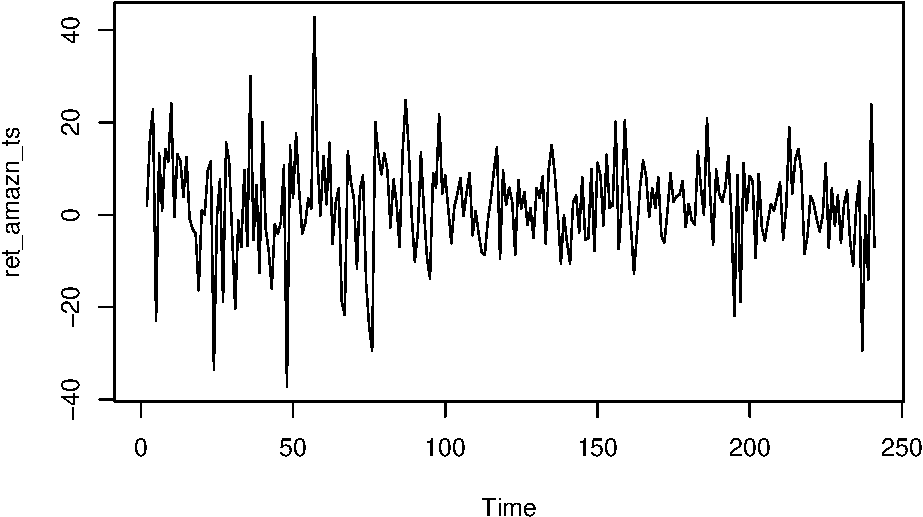
\includegraphics{06-ESTACIONARIEDAD_files/figure-latex/unnamed-chunk-4-1.pdf}

\hypertarget{estacionariedad-1}{%
\subsection{Estacionariedad}\label{estacionariedad-1}}

\begin{Shaded}
\begin{Highlighting}[]
\CommentTok{\#MA\_m5\textless{}{-}forecast::ma(ret\_amazn\_ts,order=11,centre=TRUE)}
\CommentTok{\#plot(ret\_amazn\_ts)+lines(MA\_m5, col="red", lwd=2)}
\FunctionTok{gglagplot}\NormalTok{(ret\_amazn\_ts,}\AttributeTok{lags=}\DecValTok{20}\NormalTok{,}\AttributeTok{do.lines=}\ConstantTok{FALSE}\NormalTok{,}\AttributeTok{colour=}\ConstantTok{FALSE}\NormalTok{)}\SpecialCharTok{+}\FunctionTok{theme\_light}\NormalTok{()}
\end{Highlighting}
\end{Shaded}

\begin{figure}
\centering
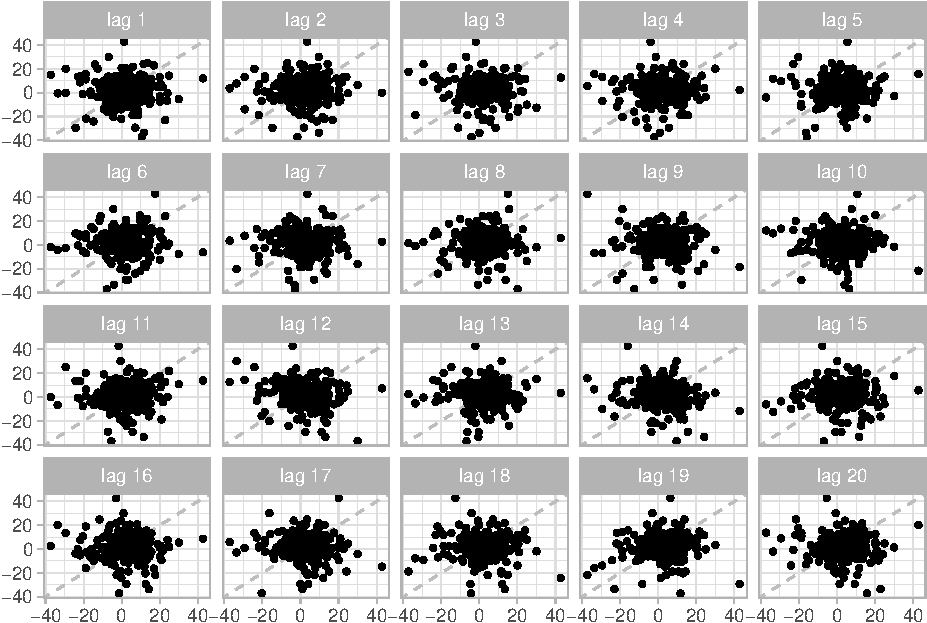
\includegraphics{06-ESTACIONARIEDAD_files/figure-latex/amazn20LAG-1.pdf}
\caption{\label{fig:amazn20LAG}Lag Plot que nos muestra la correlación entre 20 lags}
\end{figure}

\begin{Shaded}
\begin{Highlighting}[]
\NormalTok{ACF\_ret\_amazn\_ts}\OtherTok{\textless{}{-}}\FunctionTok{acf}\NormalTok{(ret\_amazn\_ts,}\AttributeTok{na.action =}\NormalTok{ na.pass)}
\end{Highlighting}
\end{Shaded}

\begin{figure}
\centering
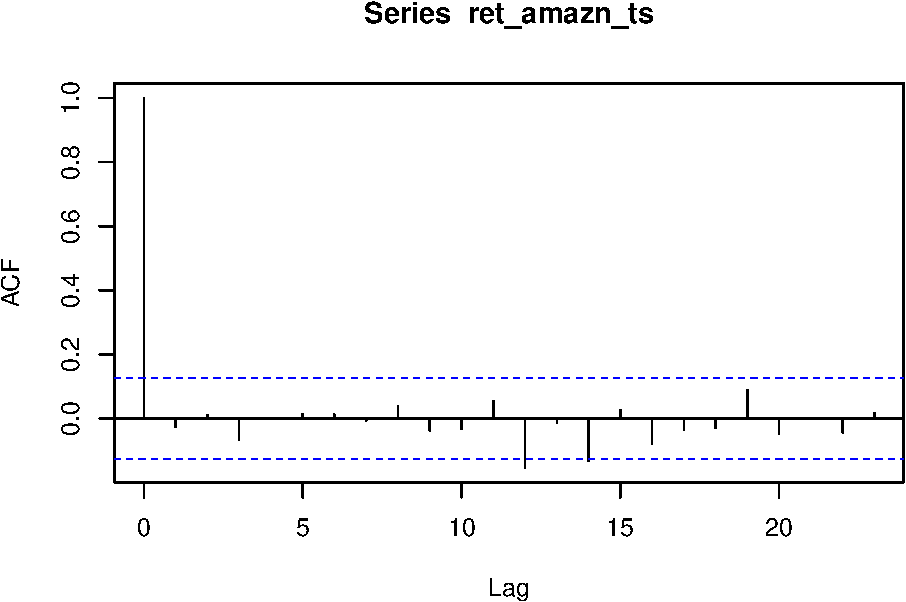
\includegraphics{06-ESTACIONARIEDAD_files/figure-latex/amazn20ACF-1.pdf}
\caption{\label{fig:amazn20ACF}Función de Autocorrelación de los retornos de AMZN en los ultimos 20 años}
\end{figure}

La Figura \ref{fig:amazn20LAG} nos idica la manera en la que se
correlacionan los lags, evidentemente no se puede ver ningún tipo de
correlacioo1ón visible. Similarmente la Figura \ref{fig:amazn20ACF} en
donde se muestra la función de autocorrelación. Expecto al primer lag
--que muestra correlacion debido a que se esta comparando consigo
mismo-- es evidente que no hay correlacioo1ón fuerte entre ninguno de
los lags. Por lo mismo, sería difícil poder encontrar y estimar valores
futuros debido a que la Figura \ref{fig:amazn20LAG} y la Figura
\ref{fig:amazn20ACF} indican que la serie de tiempo de los retornos de
AMZN de la Figura \ref{fig:amazn20} es \textbf{completamente aleatorio y no
hay estacionariedad}.

\hypertarget{procesos-estacionarios-univariados}{%
\chapter{Procesos estacionarios univariados}\label{procesos-estacionarios-univariados}}

En este capítulo analizaremos el método o metodología de análisis de
series de tiempo propuesto por Box y Jenkins (1970). Los modelos
propuestos dentro de está metodología o conjunto de métodos se han
vuelto indispensables para efectos de realizar pronósticos de corto
plazo.

En este sentido, se analizarán los métodos más importantes en series de
tiempo: Autoregresivos (AR) y de Medias Móviles (MA). Asimismo, se
realizará un análisis de los procesos que resultan de la combinación de
ambos, conocida como ARMA, los cuales son más comúnmente usados para
realizar pronósticos.

\hypertarget{procesos-autoregresivos-ar}{%
\section{Procesos Autoregresivos (AR)}\label{procesos-autoregresivos-ar}}

Los procesos autoregresivos tienen su origen en el trabajo de Cochrane y
Orcutt de 1949, mediante el cual analizaron los residuales de una
regresión clásica como un proceso autoregresivo. Puede consultarse el
apéndice para la discusión del modelo de regresión clásica.

\hypertarget{ar1}{%
\subsection{AR(1)}\label{ar1}}

Como primer caso analizaremos al proceso autoregresivo de primer orden,
\(AR(1)\), el cual podemos definir como una Ecuación Lineal en Diferencia
Estocástica de Primer Orden. Diremos que una Ecuación Lineal en
Diferencia de Primer Orden es estocástica si en su representación
analítica considera un componente estocástico como en la ecuación
\eqref{eq:EDOEst1} descrita a continuación:

\begin{equation}
    X_t = a_0 + a_1 X_{t-1} + U_t
\label{eq:EDOEst1}
\end{equation}

Donde \(a_0\) es un término constante, \(U_t\) es un proceso estacionario,
con media cero (0), una varianza finita y constante (\(\sigma^2\)) y una
covarianza que depende de la distancia entre \(t\) y cualquier \(t-s\)
(\(\gamma_s\))--que no depende de los valores pasados o futuros de la
variable--, \(X_0\) es el valor inicial de \(X_t\). No obstante, en general
vamos a asumir que la covarianza será cero (0), por lo que tendremos un
proceso puramente aleatorio. Considerando la ecuación \eqref{eq:EDOEst1} y
un proceso de sustitución sucesivo podemos establecer lo siguiente,
empezando con \(X_1\): \begin{eqnarray*}
    X_{1} & = & a_0 + a_1 X_{0} + U_{1}
\end{eqnarray*}

Para \(X_2\): \begin{eqnarray*}
X_{2} & = & a_0 + a_1 X_{1} + U_{2} \\
    & = & a_0 + a_1 (a_0 + a_1 X_{0} + U_{1}) + U_{2} \\
    & = & a_0 + a_1 a_0 + a_1^2 X_{0} + a_1 U_{1} + U_{2}
\end{eqnarray*}

Para \(X_3\): \begin{eqnarray*}
X_{3} & = & a_0 + \alpha X_{2} + U_{3} \\
    & = & a_0 + a_1 (a_0 + a_1 a_0 + a_1^2 X_{0} + a_1 U_{1} + U_{2}) + U_{3} \\
    & = & a_0 + a_1 a_0 + a_1^2 a_0 + a_1^3 X_{0} + a_1^2 U_{1} + a_1 U_{2} + U_{3}
\end{eqnarray*}

Así, para cualquier \(X_t\), \(t = 1, 2, 3, \ldots\), obtendríamos:
\begin{eqnarray}
X_{t} & = & a_0 + a_1 X_{t - 1} + U_{t} \nonumber \\
    & = & a_0 + a_1 (a_0 + a_1 a_0 + a_1^2 a_0 + \ldots + a_1^{t-2} a_0 + a_1^{t-1} X_{0} \nonumber \\
    &   & + a_1^{t-2} U_{1} + \ldots + a_1 U_{t - 2} + U_{t - 1}) + U_{t} \nonumber \\
    & = & a_0 + a_1 a_0 + a_1^2 a_0 + a_1^3 a_0 + \ldots + a_1^{t-1} a_0 + a_1^{t} X_{0} \nonumber \\
    &   & + a_1^{t-1} U_{1} + \ldots a_1^2 U_{t - 2} + a_1 U_{t - 1} + U_{t} \nonumber \\
    & = & (1 + a_1 + a_1^2 + a_1^3 + \ldots + a_1^{t-1}) a_0 + a_1^{t} X_{0} \nonumber \\
    &   & + a_1^{t-1} U_{1} + \ldots + a_1^2 U_{t - 2} + a_1 U_{t - 1} + U_{t}  \nonumber\\
    & = & \frac{1 - a_1^t}{1 - a_1} a_0 + a_1^{t} X_{0} + \sum^{t-1}_{j = 0} a_1^{j} U_{t - j} 
    \label{eq:EDOSSol}
\end{eqnarray}

De esta forma en la ecuación \eqref{eq:EDOSSol} observamos un proceso que
es explicado por dos partes: una que depende del tiempo y otra que
depende de un proceso estocástico. Asimismo, debe notarse que la
condición de convergencia es idéntica que en el caso de ecuaciones en
diferencia estudiadas al inicio del curso: \(\lvert a_1 \lvert < 1\), por
lo que cuando \(t \to \infty\), la expresión \eqref{eq:EDOSSol} será la
siguiente:

\begin{equation}
    X_t = \frac{1}{1 - a_1} a_0 + \sum^{\infty}_{j = 0} a_1^{j} U_{t - j}
    \label{eq:EDOSLP}
\end{equation}

Así, desaparece la parte dependiente del tiempo y únicamente prevalece
la parte que es dependiente del proceso estocástico. Esta es la solución
de largo plazo del proceso \(AR(1)\), la cual depende del proceso
estocástico. Notemos, además, que esta solución implica que la variable
o la serie de tiempo \(X_t\) es tambien un proceso estocástico que hereda
las propiedades de \(U_t\). Así, \(X_t\) es también un proceso estocástico
estacionario, como demostraremos más adelante.

Observemos que la ecuación \eqref{eq:EDOSLP} se puede reescribir si
consideramos la formulación que en la literatura se denomina como la
descomposición de Wold, en la cual se define que es posible asumir que
\(\psi_j = a_1^j\) y se considera el caso en el cual
\(\lvert a_1 \lvert< 1\), de esta forma tendremos que por ejemplo cuando:
\begin{equation*}
    \sum^{\infty}_{j = 0} \psi^2_j = \sum^{\infty}_{j = 0} a_1^{2j} = \frac{1}{1 - a_1^2} 
\end{equation*}

Alternativamente y de forma similar a las ecuaciones en diferencia
estudiadas previamente podemos escribir el proceso \(AR(1)\) mediante el
uso del operador rezago como:

\begin{eqnarray}
    X_t & = & a_0 + a_1 L X_t + U_t \nonumber \\
    X_t - a_1 L X_t & = & a_0 + U_t \nonumber \\
    (1 - a_1 L) X_t & = & a_0 + U_t \nonumber \\
    X_t & = & \frac{a_0}{1 - a_1 L} + \frac{1}{1 - a_1 L} U_t
    \label{eq:AR1}
\end{eqnarray}

En esta última ecuación retomamos el siguiente término para reescribirlo
como:

\begin{equation}
    \frac{1}{1 - a_1 L} = 1 + a_1 L + a_1^2 L^2 + a_1^3 L^3 + \ldots
    \label{eq:AR2}
\end{equation}

Tomando este resultado para sustituirlo en ecuación \eqref{eq:AR1},
obtenemos la siguiente expresión:

\begin{eqnarray}
X_t & = & (1 + a_1 L + a_1^2 L^2 + a_1^3 L^3 + \ldots) a_0 + (1 + a_1 L + a_1^2 L^2 + a_1^3 L^3 + \ldots) U_t \nonumber \\
    & = & (1 + a_1 + a_1^2 + a_1^3 + \ldots) a_0 + U_t + a_1 U_{t-1} + a_1^2 U_{t-2} + a_1^3 U_{t-3} + \ldots \nonumber \\
    & = & \frac{a_0}{1 - a_1} + \sum^{\infty}_{j = 0} a_1^j U_{t-j}
    \label{eq:AR1Sol}
\end{eqnarray}

Donde la condición de convergencia y estabilidad del proceso descrito en
esta ecuación es que \(\lvert a_1 \lvert < 1\). Por lo que hemos
demostrado que mediante el uso del operador de rezago es posible llegar
al mismo resultado que obtuvimos mediante el procedimiento de
sustituciones iterativas.

La ecuación \eqref{eq:AR1Sol} se puede interpretar como sigue. La
solución o trayectoria de equilibrio de un AR(1) se divide en dos
partes. La primera es una constante que depende de los valores de \(a_0\)
y \(a_1\). La segunda parte es la suma ponderada de las desviaciones o
errores observados y acumulados en el tiempo hasta el momento \(t\).

Ahora obtendremos los momentos que describen a la serie de tiempo cuando
se trata de un porceso \(AR(1)\). Para ello debemos obtener la media, la
varianza y las covarianzas de \(X_t\). Para los siguientes resultados
debemos recordar y tener en mente que si \(U_t\) es un proceso puramente
aleatorio, entonces:

\begin{enumerate}
\def\labelenumi{\arabic{enumi}.}
\tightlist
\item
  \(\mathbb{E}[U_t] = 0\) para todo \(t\)
\item
  \(Var[U_t] = \sigma^2\) para todo \(t\)
\item
  \(Cov[U_t, U_s] = 0\) para todo \(t \neq s\)
\end{enumerate}

Dicho lo anterior y partiendo de la ecuación \eqref{eq:AR1Sol}, el primer
momento o valor esperado de la serie de tiempo será el siguiente:
\begin{eqnarray}
\mathbb{E}[X_t] & = & \mathbb{E} \left[ \frac{a_0}{1 - a_1} + \sum^{\infty}_{j = 0} a_1^j U_{t-j} \right] \nonumber \\
    & = & \frac{a_0}{1 - a_1} + \sum^{\infty}_{j = 0} a_1^j \mathbb{E}[U_{t-j}] \nonumber \\
    & = & \frac{a_0}{1 - a_1} = \mu
    \label{eq:AR1m1}
\end{eqnarray}

Respecto de la varianza podemos escribir la siguiente expresión a partir
de la ecuación \eqref{eq:AR1Sol}:

\begin{eqnarray}
Var[X_t] & = & \mathbb{E}[(X_t - \mu)^2] \nonumber \\
    & = & \mathbb{E} \left[ \left( \frac{a_0}{1 - a_1} + \sum^{\infty}_{j = 0} a_1^j U_{t-j} - \frac{a_0}{1 - a_1} \right)^2 \right] \nonumber \\
    & = & \mathbb{E}[(U_{t} + a_1 U_{t-1} + a_1^2 U_{t-2} + a_1^3 U_{t-3} + \ldots)^2] \nonumber \\
    & = & \mathbb{E}[U^2_{t} + a_1^2 U^2_{t-1} + a_1^4 U^2_{t-2} + a_1^6 U^2_{t-3} + \ldots \nonumber \\
    &   & + 2 a_1 U_t U_{t-1} + 2 a_1^2 U_t U_{t-2} + \ldots] \nonumber \\
    & = & \mathbb{E}[U^2_{t}] + a_1^2 \mathbb{E}[U^2_{t-1}] + a_1^4 \mathbb{E}[U^2_{t-2}] + a_1^6 \mathbb{E}[U^2_{t-3}] + \ldots \nonumber \\
    & = & \sigma^2 + a_1^2 \sigma^2 + a_1^4 \sigma^2 + a_1^6 \sigma^2 + \ldots \nonumber \\
    & = & \sigma^2 (1 + a_1^2 + a_1^4 + a_1^6 + \ldots) \nonumber \\
    & = & \sigma^2 \frac{1}{1 - a_1^2} = \gamma(0)
    \label{eq:AR1Var}
\end{eqnarray}

Previo a analizar la covarianza de la serie recordemos que para el
proceso puramente aleatorio \(U_t\) su varianza y covarianza puede verse
como \(\mathbb{E}[U_t, U_s] = \sigma^2\), para \(t = s\), y
\(\mathbb{E}[U_t, U_s] = 0\), para cualquier otro caso, respectivamente.

Dicho lo anterior, partiendo de la ecuación \eqref{eq:AR1Sol} la
covarianza de la serie estará dada por:

\begin{eqnarray}
Cov(X_t, X_{t-\tau}) & = & \mathbb{E}[(X_t - \mu)(X_{t-\tau} - \mu)] \nonumber \\
    & = & \mathbb{E} \left[ \left( \frac{a_0}{1 - a_1} + \sum^{\infty}_{j = 0} a_1^j U_{t-j} - \frac{a_0}{1 - a_1} \right) \right. \nonumber \\
    &   & \left. \times \left( \frac{a_0}{1 - a_1} + \sum^{\infty}_{j = 0} a_1^j U_{t-\tau-j} - \frac{a_0}{1 - a_1} \right) \right] \nonumber \\
    & = & a_1^{\tau} \mathbb{E}[U^2_{t-\tau} + a_1 U^2_{t-\tau-1} + a_1^2 U^2_{t-\tau-2} + a_1^3 U^2_{t-\tau-3} + \ldots] \nonumber \\
    & = & a_1^{\tau} \sigma^2 \frac{1}{1 - a_1^2} = \gamma(\tau)
    \label{eq:AR1Cov}
\end{eqnarray}

Notése que con estos resultados en las ecuaciones \eqref{eq:AR1Var} y
\eqref{eq:AR1Cov} podemos construir la función de autocorrelación teórica
como sigue:

\begin{eqnarray}
\rho(\tau) & = & \frac{\gamma(\tau)}{\gamma(0)} \nonumber \\
    & = & a_1^\tau
    \label{eq:emi1}
\end{eqnarray}

Donde \(\tau = 1, 2, 3, \ldots\) y \(\lvert a_1 \lvert < 1\). Este último
resultado significa que cuando el proceso autoregresivo es de orden 1
(es decir, AR(1)) la función de autocorrelación teóricamente es igual al
parámetro \(a_1\) elevado al número de rezagos considerados. No obstante,
note que esto no significa que la autocorrelación observada sea como lo
expresa en planteamiento anterior. Por el contrario, una observación
sencilla mostraría que la autocorrelación observada sería ligeramente
distinta a la autocorrelación teórica.

Ahora veámos algunos ejemplos. En el primer ejemplo simularemos una
serie y mostraremos el analísis de un proceso construído considerando un
proceso puramente aleatorio como componente \(U_t\).\footnote{El procedimiento e implementación del ejercicio
  está en el archivo R denominado Clase 4 del repositorio de GitHub.}
Por su parte, en un segundo ejemplo aplicaremos el análisis a una serie
de tiempo de una variable económica observada.\footnote{El procedimiento e implementación del ejercicio
  está en el archivo R denominado Clase 5 del repositorio de GitHub.}

Para el primer ejemplo consideremos un proceso dado por la forma de un
\(AR(1)\) como en la ecuación \eqref{eq:AR1} cuya solución esta dada por la
ecuación \eqref{eq:AR1Sol}. En especifico, supongamos que el término o
componente estocástico \(U_t\) es una serie generada a partir de numeros
aleatorios de una función normal con media \(0\) y desviación estándar
\(4\). Los detalles del proceso simulado se muestra en las siguientes
gráficas.

\hypertarget{ejemplo-ar1}{%
\subsubsection{EJEMPLO AR(1)}\label{ejemplo-ar1}}

\begin{Shaded}
\begin{Highlighting}[]
\FunctionTok{library}\NormalTok{(ggplot2)}
\FunctionTok{library}\NormalTok{(dplyr)}
\FunctionTok{library}\NormalTok{(readxl)}
\FunctionTok{library}\NormalTok{(latex2exp)}

\CommentTok{\# Parametros:}
\NormalTok{a0 }\OtherTok{\textless{}{-}} \DecValTok{5}\NormalTok{; a1 }\OtherTok{\textless{}{-}} \FloatTok{0.9}\NormalTok{; X\_0 }\OtherTok{\textless{}{-}}\NormalTok{ (a0}\SpecialCharTok{/}\NormalTok{(}\DecValTok{1} \SpecialCharTok{{-}}\NormalTok{ a1)); T }\OtherTok{\textless{}{-}} \DecValTok{1000}
\end{Highlighting}
\end{Shaded}

Por lo tanto tenemos la serie de tiempo \(AR(1)\):
\[ X_t= 5+0.9X_{t-1}+U_t\]

\begin{Shaded}
\begin{Highlighting}[]
\CommentTok{\# Definimos un data frame para almacenar el proceso, agregamos una columna para el tiempo}
\NormalTok{X\_t }\OtherTok{\textless{}{-}} \FunctionTok{data.frame}\NormalTok{(}\AttributeTok{Tiempo =} \FunctionTok{c}\NormalTok{(}\DecValTok{0}\SpecialCharTok{:}\NormalTok{T))}

\CommentTok{\#  Parte estocastica de la serie de tiempo:}
\FunctionTok{set.seed}\NormalTok{(}\DecValTok{12345}\NormalTok{)}

\CommentTok{\# Agregamos un término estocástico al data frame}
\NormalTok{X\_t}\SpecialCharTok{$}\NormalTok{U\_t }\OtherTok{\textless{}{-}} \FunctionTok{rnorm}\NormalTok{(T}\SpecialCharTok{+}\DecValTok{1}\NormalTok{, }\AttributeTok{mean =} \DecValTok{0}\NormalTok{, }\AttributeTok{sd =} \DecValTok{4}\NormalTok{)}
\end{Highlighting}
\end{Shaded}

En este caso el termino estocastico tiene una media de \(0\) y una
desviación estándar constante \(\sigma^2=4\)

\begin{Shaded}
\begin{Highlighting}[]
\CommentTok{\# Agregamos columnas con NA\textquotesingle{}s para un proceso teorico y uno real}
\NormalTok{X\_t}\SpecialCharTok{$}\NormalTok{X\_t }\OtherTok{\textless{}{-}} \ConstantTok{NA}
\NormalTok{X\_t}\SpecialCharTok{$}\NormalTok{XR\_t }\OtherTok{\textless{}{-}} \ConstantTok{NA}

\CommentTok{\# La serie teórica inicia en un valor inicial X\_0}
\NormalTok{X\_t}\SpecialCharTok{$}\NormalTok{X\_t[}\DecValTok{1}\NormalTok{] }\OtherTok{\textless{}{-}}\NormalTok{ X\_0}

\CommentTok{\# La serie real inicia en un valor inicial X\_0}
\NormalTok{X\_t}\SpecialCharTok{$}\NormalTok{XR\_t[}\DecValTok{1}\NormalTok{] }\OtherTok{\textless{}{-}}\NormalTok{ X\_0}

\CommentTok{\# Agregamos una columna para la función de Autocorrelación teórica:}
\NormalTok{X\_t}\SpecialCharTok{$}\NormalTok{rho }\OtherTok{\textless{}{-}}\ConstantTok{NA}

\ControlFlowTok{for}\NormalTok{ (i }\ControlFlowTok{in} \DecValTok{2}\SpecialCharTok{:}\NormalTok{(T }\SpecialCharTok{+} \DecValTok{1}\NormalTok{)) \{}
  \CommentTok{\# Real:}
\NormalTok{  X\_t}\SpecialCharTok{$}\NormalTok{XR\_t[i] }\OtherTok{=}\NormalTok{ a0 }\SpecialCharTok{+}\NormalTok{ a1}\SpecialCharTok{*}\NormalTok{X\_t}\SpecialCharTok{$}\NormalTok{XR\_t[i}\DecValTok{{-}1}\NormalTok{] }\SpecialCharTok{+}\NormalTok{ X\_t}\SpecialCharTok{$}\NormalTok{U\_t[i}\DecValTok{{-}1}\NormalTok{]}
  
  \CommentTok{\# Teórico:}
\NormalTok{  X\_t}\SpecialCharTok{$}\NormalTok{X\_t[i] }\OtherTok{=}\NormalTok{ X\_t}\SpecialCharTok{$}\NormalTok{X\_t[i}\DecValTok{{-}1}\NormalTok{] }\SpecialCharTok{+}\NormalTok{ (a1}\SpecialCharTok{\^{}}\NormalTok{(i}\DecValTok{{-}1}\NormalTok{))}\SpecialCharTok{*}\NormalTok{X\_t}\SpecialCharTok{$}\NormalTok{U\_t[i}\DecValTok{{-}1}\NormalTok{]}
  
  \CommentTok{\# Autocorrelación:}
\NormalTok{  X\_t}\SpecialCharTok{$}\NormalTok{rho[i}\DecValTok{{-}1}\NormalTok{] }\OtherTok{=}\NormalTok{ a1}\SpecialCharTok{\^{}}\NormalTok{(i}\DecValTok{{-}1}\NormalTok{)}
\NormalTok{\}}

\FunctionTok{head}\NormalTok{(X\_t)}
\CommentTok{\#\textgreater{}   Tiempo        U\_t      X\_t     XR\_t      rho}
\CommentTok{\#\textgreater{} 1      0  2.3421153 50.00000 50.00000 0.900000}
\CommentTok{\#\textgreater{} 2      1  2.8378641 52.10790 52.34212 0.810000}
\CommentTok{\#\textgreater{} 3      2 {-}0.4372133 54.40657 54.94577 0.729000}
\CommentTok{\#\textgreater{} 4      3 {-}1.8139887 54.08785 54.01398 0.656100}
\CommentTok{\#\textgreater{} 5      4  2.4235498 52.89769 51.79859 0.590490}
\CommentTok{\#\textgreater{} 6      5 {-}7.2718239 54.32877 54.04228 0.531441}
\end{Highlighting}
\end{Shaded}

\begin{figure}

{\centering 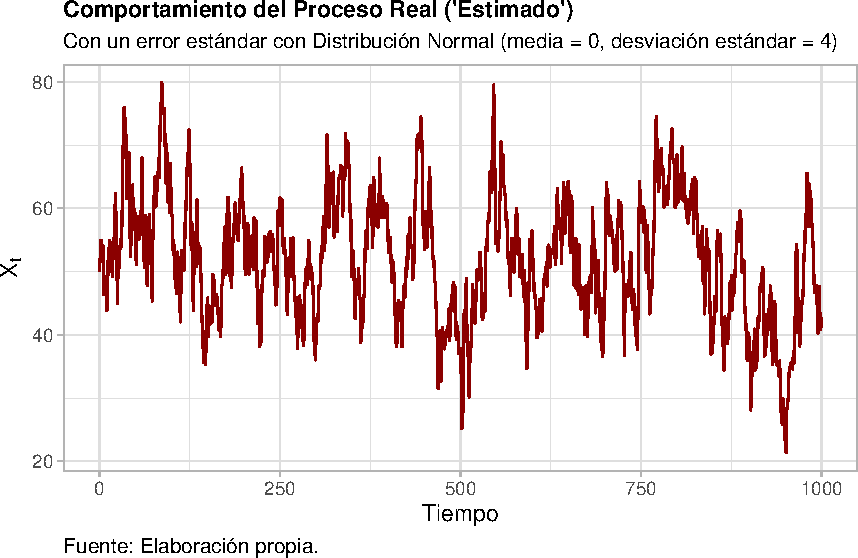
\includegraphics[width=1\linewidth]{07-PE_Univariados_files/figure-latex/GAR1Real-1} 

}

\caption{AR(1) considerando $X_t=5+0.9X_{t-1}+U_t$ ; $X_0=50$ y que $U_t$~$N(0, 4)$ y que $U_t \sim \mathcal{N}(0, 4)$}\label{fig:GAR1Real}
\end{figure}

\begin{Shaded}
\begin{Highlighting}[]

\FunctionTok{ggplot}\NormalTok{(}\AttributeTok{data =}\NormalTok{ X\_t, }\FunctionTok{aes}\NormalTok{(}\AttributeTok{x =}\NormalTok{ Tiempo, }\AttributeTok{y =}\NormalTok{ X\_t)) }\SpecialCharTok{+} 
  \FunctionTok{geom\_line}\NormalTok{(}\AttributeTok{size =} \FloatTok{0.5}\NormalTok{, }\AttributeTok{color =} \StringTok{"\#0F531C"}\NormalTok{) }\SpecialCharTok{+}
  \FunctionTok{theme\_light}\NormalTok{() }\SpecialCharTok{+} 
  \FunctionTok{xlab}\NormalTok{(}\StringTok{"Tiempo"}\NormalTok{) }\SpecialCharTok{+} 
  \FunctionTok{ylab}\NormalTok{(}\FunctionTok{TeX}\NormalTok{(}\StringTok{"$X\_t$"}\NormalTok{)) }\SpecialCharTok{+} 
  \FunctionTok{theme}\NormalTok{(}\AttributeTok{plot.title =} \FunctionTok{element\_text}\NormalTok{(}\AttributeTok{size =} \DecValTok{11}\NormalTok{, }\AttributeTok{face =} \StringTok{"bold"}\NormalTok{, }\AttributeTok{hjust =} \DecValTok{0}\NormalTok{)) }\SpecialCharTok{+} 
  \FunctionTok{theme}\NormalTok{(}\AttributeTok{plot.subtitle =} \FunctionTok{element\_text}\NormalTok{(}\AttributeTok{size =} \DecValTok{10}\NormalTok{, }\AttributeTok{hjust =} \DecValTok{0}\NormalTok{)) }\SpecialCharTok{+} 
  \FunctionTok{theme}\NormalTok{(}\AttributeTok{plot.caption =} \FunctionTok{element\_text}\NormalTok{(}\AttributeTok{size =} \DecValTok{10}\NormalTok{, }\AttributeTok{hjust =} \DecValTok{0}\NormalTok{)) }\SpecialCharTok{+}
  \FunctionTok{theme}\NormalTok{(}\AttributeTok{plot.margin =} \FunctionTok{unit}\NormalTok{(}\FunctionTok{c}\NormalTok{(}\DecValTok{1}\NormalTok{,}\DecValTok{1}\NormalTok{,}\DecValTok{1}\NormalTok{,}\DecValTok{1}\NormalTok{), }\StringTok{"cm"}\NormalTok{)) }\SpecialCharTok{+}
  \FunctionTok{labs}\NormalTok{(}
    \AttributeTok{title =} \StringTok{"Comportamiento del Proceso Teórico"}\NormalTok{,}
    \AttributeTok{subtitle =} \StringTok{"Con un error con Distribución Normal (media = 0, desviación estándar = 4)"}\NormalTok{,}
    \AttributeTok{caption =} \StringTok{"Fuente: Elaboración propia."}
\NormalTok{  )}
\end{Highlighting}
\end{Shaded}

\textbackslash begin\{figure\}

\{\centering 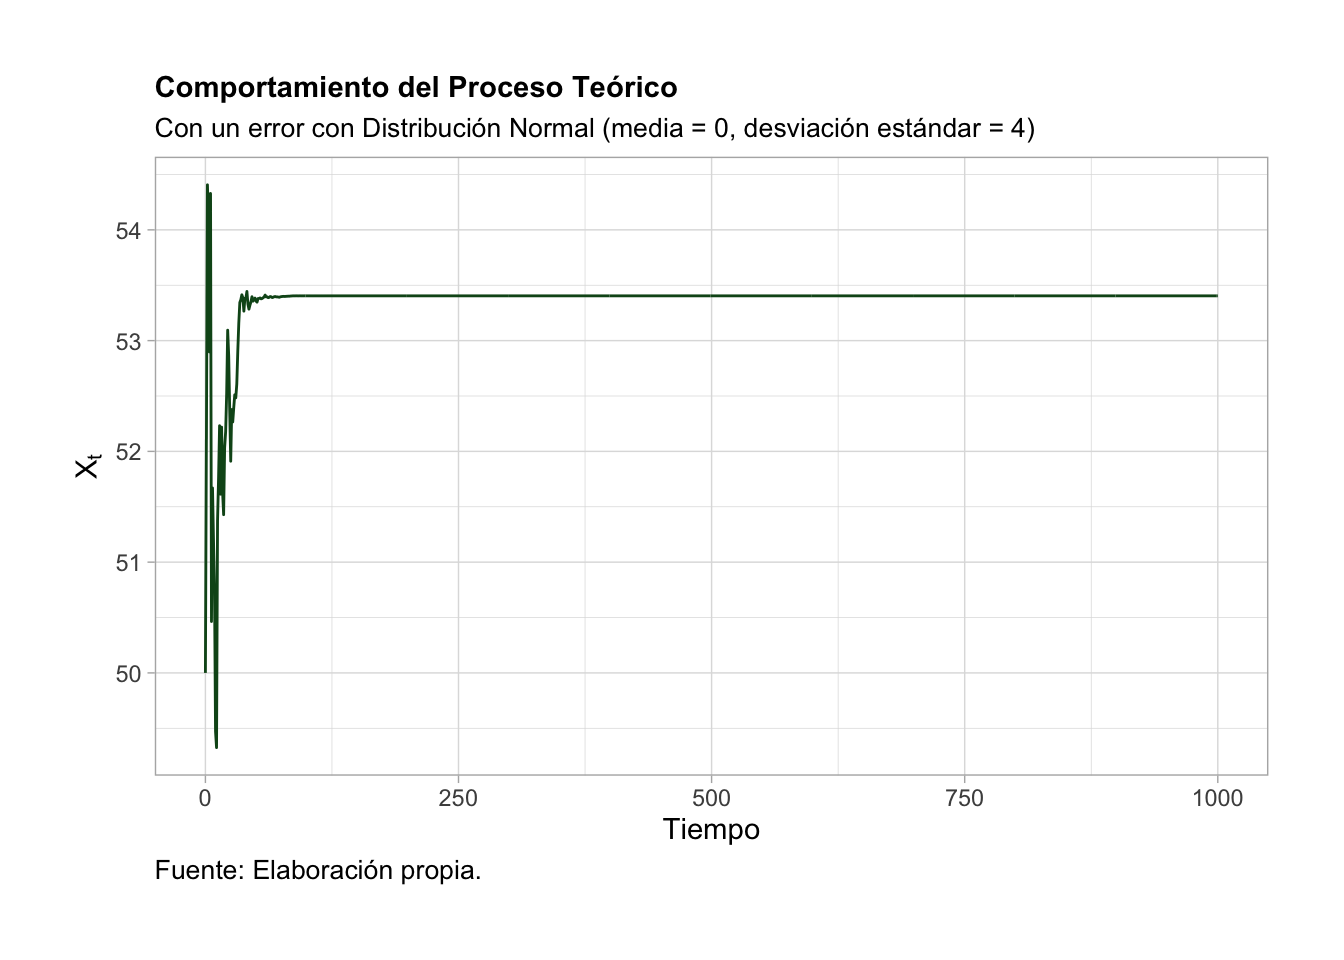
\includegraphics[width=1\linewidth]{07-PE_Univariados_files/figure-latex/GAR1Teo-1}

\}

\caption{$X_t = \frac{5}{1 - 0.9} + \sum_{j = 0}^{t-1} 0.9^j U_{t-j}$, y que $U_t \sim \mathcal{N}(0, 4)$}

\}\label{fig:GAR1Teo}
\textbackslash end\{figure\}

\begin{Shaded}
\begin{Highlighting}[]

\FunctionTok{acf}\NormalTok{(X\_t}\SpecialCharTok{$}\NormalTok{XR\_t, }\AttributeTok{lag.max =} \DecValTok{30}\NormalTok{, }\AttributeTok{col =} \StringTok{"blue"}\NormalTok{, }
    \AttributeTok{ylab =} \StringTok{"Autocorrelacion"}\NormalTok{,}
    \AttributeTok{xlab=}\StringTok{"Rezagos"}\NormalTok{, }
    \AttributeTok{main=}\StringTok{"Funcion de Autocorrelacion Real"}\NormalTok{)}
\end{Highlighting}
\end{Shaded}

\begin{figure}

{\centering 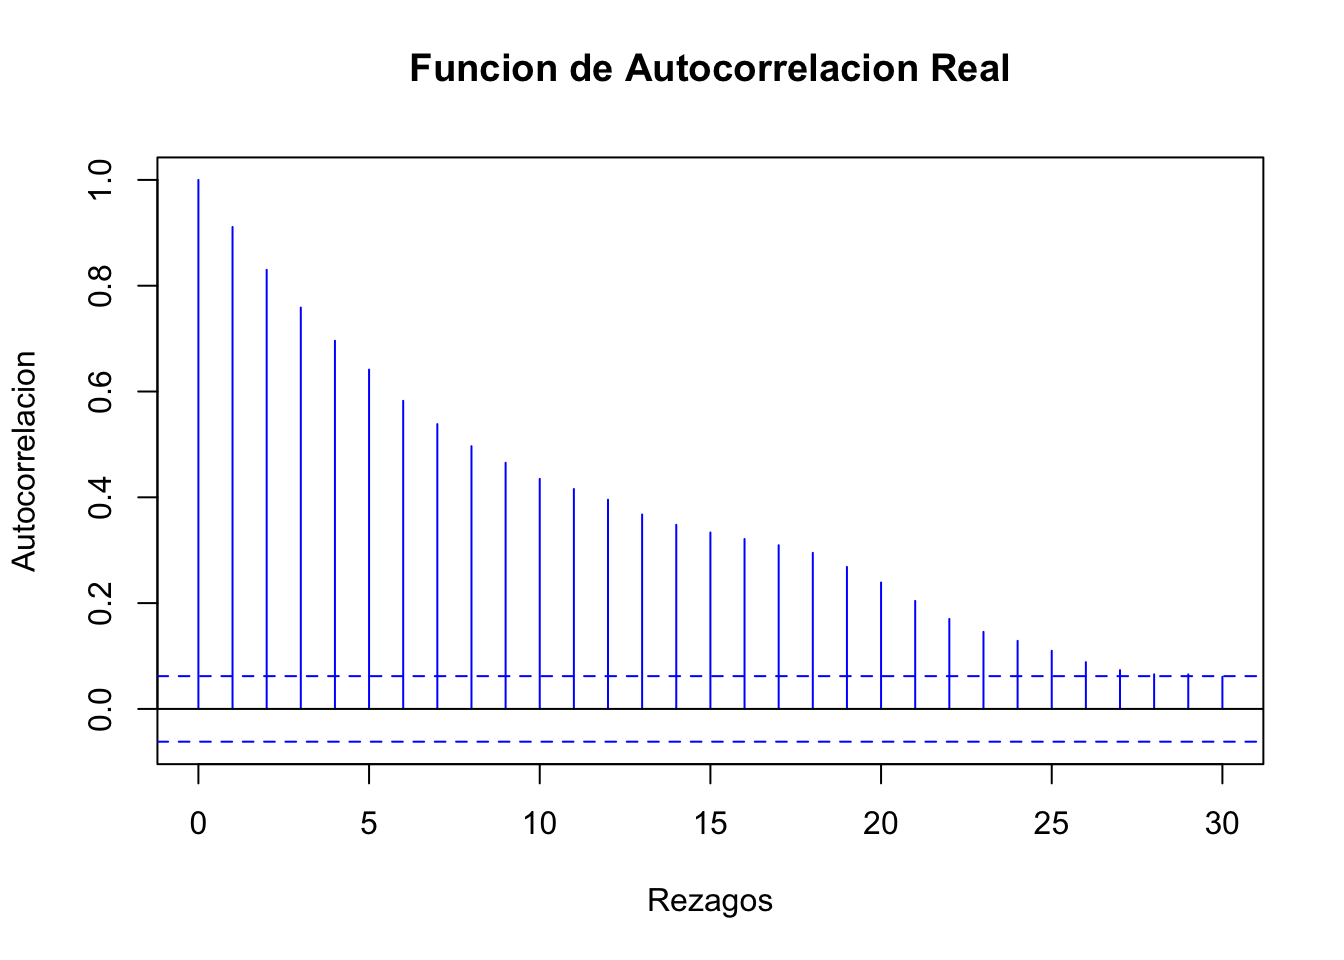
\includegraphics[width=1\linewidth]{07-PE_Univariados_files/figure-latex/GAR1FACr-1} 

}

\caption{Función de autocorrelación de un AR(1): $\rho(\tau)=\frac{\gamma(  au)}{\gamma(0)}$}\label{fig:GAR1FACr}
\end{figure}

\begin{Shaded}
\begin{Highlighting}[]

\FunctionTok{barplot}\NormalTok{(X\_t}\SpecialCharTok{$}\NormalTok{rho[}\DecValTok{1}\SpecialCharTok{:}\DecValTok{30}\NormalTok{], }\AttributeTok{names.arg =} \FunctionTok{c}\NormalTok{(}\DecValTok{1}\SpecialCharTok{:}\DecValTok{30}\NormalTok{), }\AttributeTok{col =} \StringTok{"blue"}\NormalTok{, }\AttributeTok{border=}\StringTok{"blue"}\NormalTok{, }\AttributeTok{density =} \FunctionTok{c}\NormalTok{(}\DecValTok{10}\NormalTok{,}\DecValTok{20}\NormalTok{), }
        \AttributeTok{ylab =} \StringTok{"Autocorrelacion"}\NormalTok{, }
        \AttributeTok{xlab=}\StringTok{"Rezagos"}\NormalTok{, }
        \AttributeTok{main=}\StringTok{"Funcion de Autocorrelacion Teórica"}\NormalTok{)}
\end{Highlighting}
\end{Shaded}

\begin{figure}

{\centering 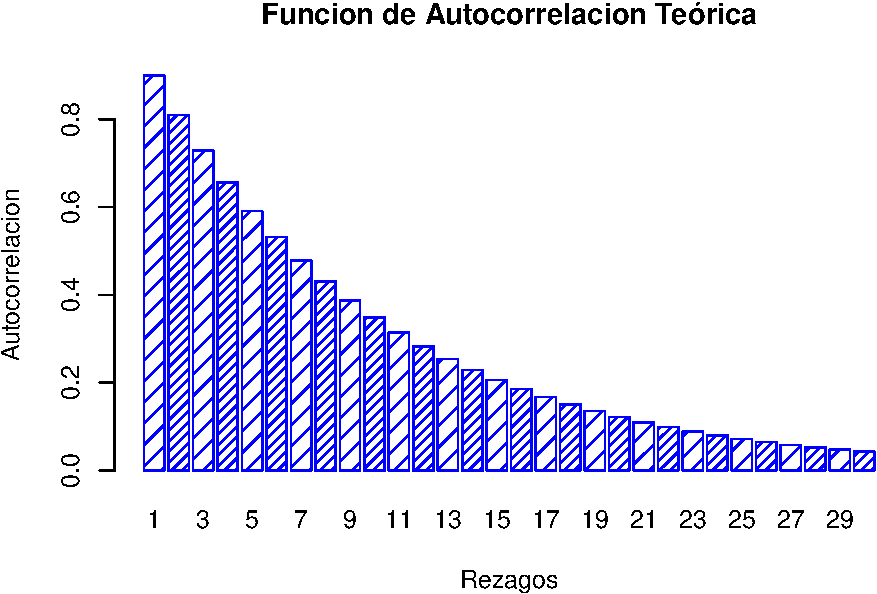
\includegraphics[width=1\linewidth]{07-PE_Univariados_files/figure-latex/GAR1FACt-1} 

}

\caption{Función de autocorrelación de un AR(1): $\rho(\tau)= a_1^\tau$}\label{fig:GAR1FACt-1}
\end{figure}

\begin{Shaded}
\begin{Highlighting}[]

\FunctionTok{acf}\NormalTok{(X\_t}\SpecialCharTok{$}\NormalTok{XR\_t, }\AttributeTok{lag.max =} \DecValTok{30}\NormalTok{, }\AttributeTok{col =} \StringTok{"blue"}\NormalTok{, }
    \AttributeTok{ylab =} \StringTok{"Autocorrelacion"}\NormalTok{,}
    \AttributeTok{xlab=}\StringTok{"Rezagos"}\NormalTok{, }
    \AttributeTok{main=}\StringTok{"Funcion de Autocorrelacion Real"}\NormalTok{)}
\end{Highlighting}
\end{Shaded}

\begin{figure}

{\centering 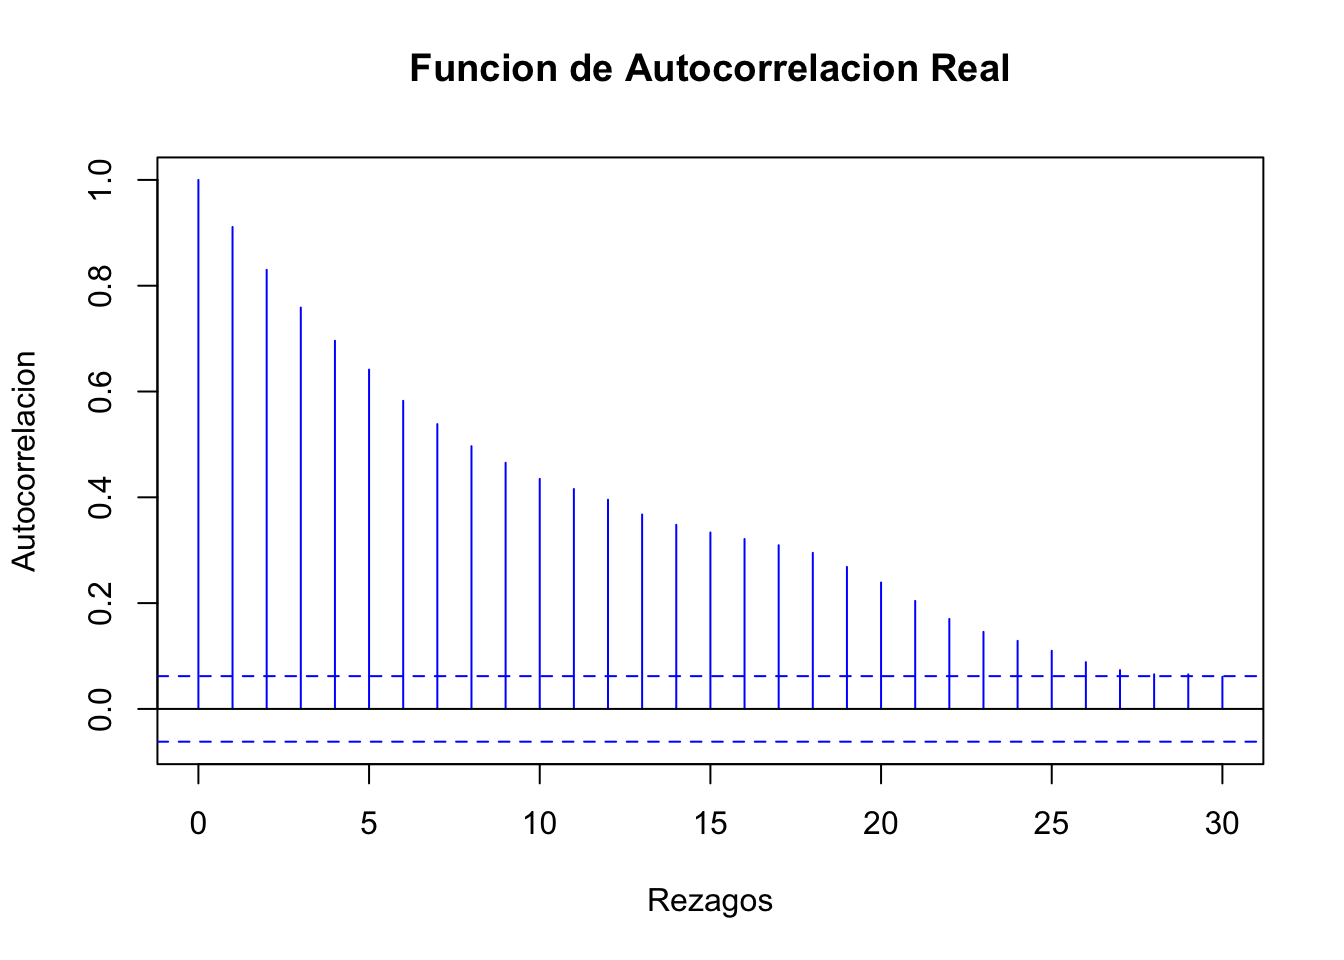
\includegraphics[width=1\linewidth]{07-PE_Univariados_files/figure-latex/GAR1FACt-2} 

}

\caption{Función de autocorrelación de un AR(1): $\rho(\tau)= a_1^\tau$}\label{fig:GAR1FACt-2}
\end{figure}

\begin{Shaded}
\begin{Highlighting}[]

\FunctionTok{ggplot}\NormalTok{(}\AttributeTok{data =}\NormalTok{ X\_t, }\FunctionTok{aes}\NormalTok{(}\AttributeTok{x =}\NormalTok{ Tiempo)) }\SpecialCharTok{+}
  \FunctionTok{geom\_line}\NormalTok{(}\FunctionTok{aes}\NormalTok{(}\AttributeTok{y =}\NormalTok{ XR\_t), }\AttributeTok{size =} \FloatTok{0.5}\NormalTok{, }\AttributeTok{color =} \StringTok{"darkred"}\NormalTok{) }\SpecialCharTok{+}
  \FunctionTok{geom\_line}\NormalTok{(}\FunctionTok{aes}\NormalTok{(}\AttributeTok{y =}\NormalTok{ X\_t), }\AttributeTok{size =} \DecValTok{1}\NormalTok{, }\AttributeTok{color =} \StringTok{"\#0F531C"}\NormalTok{) }\SpecialCharTok{+}
  \FunctionTok{theme\_bw}\NormalTok{() }\SpecialCharTok{+} 
  \FunctionTok{xlab}\NormalTok{(}\StringTok{"Tiempo"}\NormalTok{) }\SpecialCharTok{+} 
  \FunctionTok{ylab}\NormalTok{(}\FunctionTok{TeX}\NormalTok{(}\StringTok{"$X\_t$"}\NormalTok{)) }\SpecialCharTok{+} 
  \FunctionTok{theme}\NormalTok{(}\AttributeTok{plot.title =} \FunctionTok{element\_text}\NormalTok{(}\AttributeTok{size =} \DecValTok{11}\NormalTok{, }\AttributeTok{face =} \StringTok{"bold"}\NormalTok{, }\AttributeTok{hjust =} \DecValTok{0}\NormalTok{)) }\SpecialCharTok{+} 
  \FunctionTok{theme}\NormalTok{(}\AttributeTok{plot.subtitle =} \FunctionTok{element\_text}\NormalTok{(}\AttributeTok{size =} \DecValTok{10}\NormalTok{, }\AttributeTok{hjust =} \DecValTok{0}\NormalTok{)) }\SpecialCharTok{+} 
  \FunctionTok{theme}\NormalTok{(}\AttributeTok{plot.caption =} \FunctionTok{element\_text}\NormalTok{(}\AttributeTok{size =} \DecValTok{10}\NormalTok{, }\AttributeTok{hjust =} \DecValTok{0}\NormalTok{)) }\SpecialCharTok{+}
  \FunctionTok{theme}\NormalTok{(}\AttributeTok{plot.margin =} \FunctionTok{unit}\NormalTok{(}\FunctionTok{c}\NormalTok{(}\DecValTok{1}\NormalTok{,}\DecValTok{1}\NormalTok{,}\DecValTok{1}\NormalTok{,}\DecValTok{1}\NormalTok{), }\StringTok{"cm"}\NormalTok{)) }\SpecialCharTok{+}
  \FunctionTok{labs}\NormalTok{(}
    \AttributeTok{title =} \StringTok{"Comportamiento de los Procesos Real y Teórico"}\NormalTok{,}
    \AttributeTok{subtitle =} \StringTok{"Con un error con Distribución Normal (media = 0, desviación estándar = 4)"}\NormalTok{,}
    \AttributeTok{caption =} \StringTok{"Fuente: Elaboración propia."}
\NormalTok{  )}
\end{Highlighting}
\end{Shaded}

\begin{figure}

{\centering 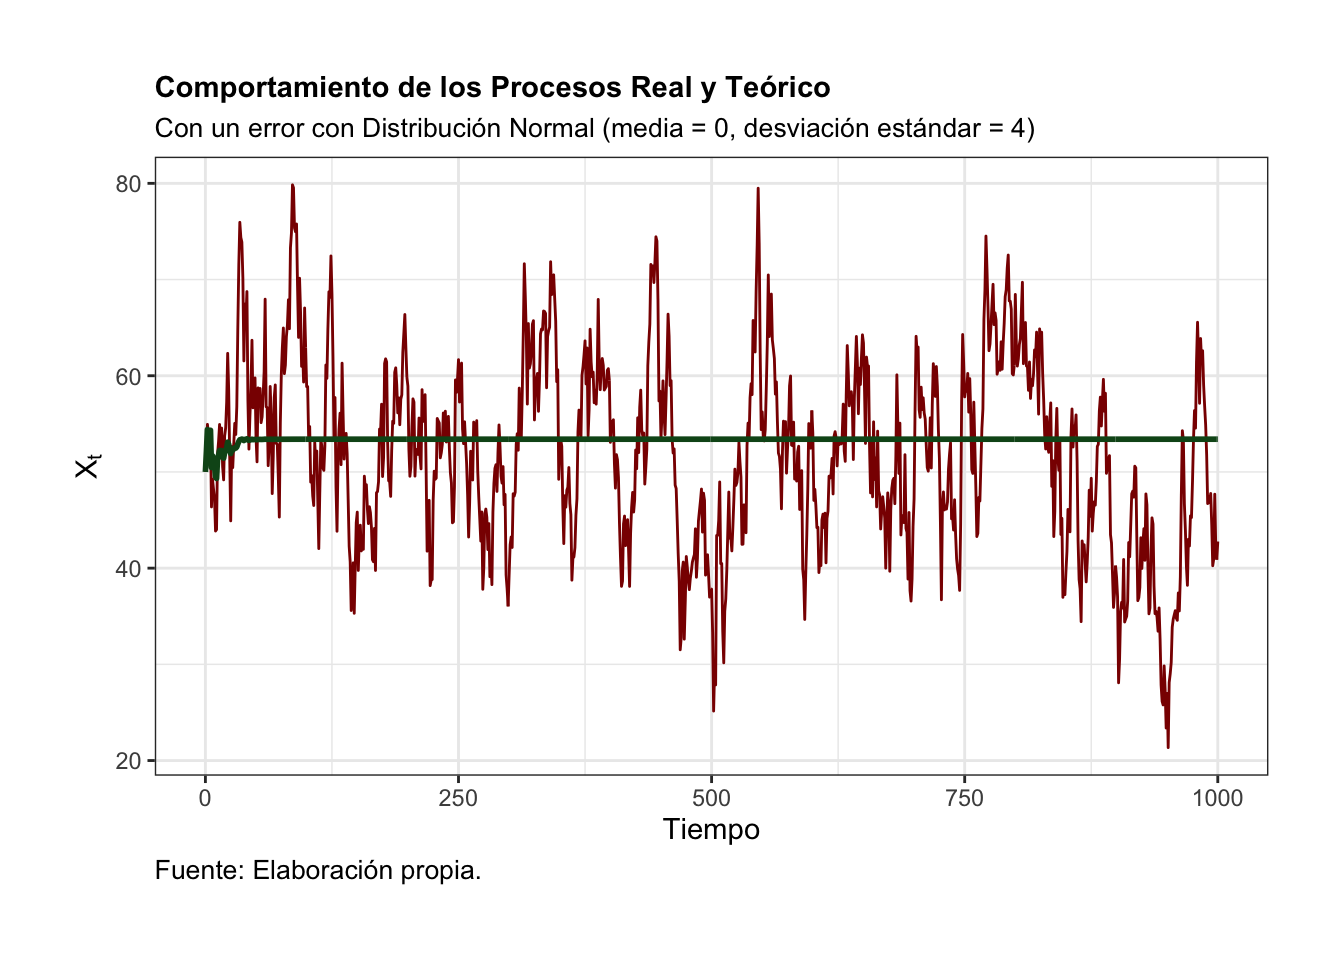
\includegraphics[width=1\linewidth]{07-PE_Univariados_files/figure-latex/GAR1Com-1} 

}

\caption{AR(1) considerando en conjunto $X_t = 5 + 0.9 X_{t-1} + U_t$; $X_0 = 50$ y $X_t = \frac{5}{1 - 0.9} + \sum_{j = 0}^{t-1} 0.9^j U_{t-j}$, y que $U_t \sim \mathcal{N}(0, 4)$}\label{fig:GAR1Com}
\end{figure}

La Figura \ref{fig:GAR1Real} ilustra el comportamiento que se debería
observar en una serie considerando el procedimiento iterativo de
construcción. Por su parte, la Figura \ref{fig:GAR1Teo} ilustra el
proceso o trayectoria de la solución de la serie de tiempo. Finalmente,
las Figuras \ref{fig:GAR1FACr} y \ref{fig:GAR1FACr} muestran el
correlograma calculado considerando una función de autocorrelación
aplicada al porceso real y una función de autocorrelación aplicada al
proceso teórico, respectivamente.

Recordemos que una trayectoria de equilibrio o solución de un \(AR(1)\) es
como se muestra en la ecuación \eqref{eq:AR1Sol}. Así, nuestra serie
simulada cumple con la característica de que los errores son más
relevantes cuando la serie es corta. Por el contrario, los errores son
menos relevantes, cuando la serie es muy larga. La Figura
\ref{fig:GAR1Com} ilustra esta observación de la trayectoria de
equilibrio.

\hypertarget{ar2}{%
\subsection{AR(2)}\label{ar2}}

Una vez analizado el caso de \(AR(1)\) analizaremos el caso del \(AR(2)\).
La ecuación generalizada del proceso autoregresivo de orden 2 (denotado
como \(AR(2)\)) puede ser escrito como:

\begin{equation}
    X_t = a_0 + a_1 X_{t-1} + a_2 X_{t-2} + U_t
    \label{eq:AR2Eq}
\end{equation}

Para el segundo ejemplo consideremos una aplicación a una serie de
tiempo en especifico:

\hypertarget{ejemplo-ar2}{%
\subsubsection{EJEMPLO AR(2)}\label{ejemplo-ar2}}

Recordando el tema pasado y la serie en la que evaluamos los cambios de
precio del ACTIVO AMZN como si fueran retornos:

\begin{Shaded}
\begin{Highlighting}[]
\CommentTok{\#install.packages("pacman")}
\CommentTok{\#pacman nos permite cargar varias librerias en una sola línea}
\FunctionTok{library}\NormalTok{(pacman)}
\NormalTok{pacman}\SpecialCharTok{::}\FunctionTok{p\_load}\NormalTok{(tidyverse,BatchGetSymbols,ggplot2,lubridate,readxl,forecast,stats,stargazer)}
\end{Highlighting}
\end{Shaded}

\begin{Shaded}
\begin{Highlighting}[]
\CommentTok{\#Primero determinamos el lapso de tiempo}
\NormalTok{pd}\OtherTok{\textless{}{-}}\FunctionTok{Sys.Date}\NormalTok{()}\SpecialCharTok{{-}}\NormalTok{(}\DecValTok{365}\SpecialCharTok{*}\DecValTok{20}\NormalTok{) }\CommentTok{\#primer fecha}
\NormalTok{pd}
\CommentTok{\#\textgreater{} [1] "2002{-}10{-}02"}
\NormalTok{ld}\OtherTok{\textless{}{-}}\FunctionTok{Sys.Date}\NormalTok{() }\CommentTok{\#última fecha}
\NormalTok{ld}
\CommentTok{\#\textgreater{} [1] "2022{-}09{-}27"}
\CommentTok{\#Intervalos de tiempo}
\NormalTok{int}\OtherTok{\textless{}{-}}\StringTok{"monthly"}
\CommentTok{\#Datos a elegir}
\NormalTok{dt}\OtherTok{\textless{}{-}}\FunctionTok{c}\NormalTok{(}\StringTok{"AMZN"}\NormalTok{)}
\CommentTok{\#Descargando los valores}
\NormalTok{data1}\OtherTok{\textless{}{-}} \FunctionTok{BatchGetSymbols}\NormalTok{(}\AttributeTok{tickers =}\NormalTok{ dt,}
                       \AttributeTok{first.date =}\NormalTok{ pd,}
                       \AttributeTok{last.date =}\NormalTok{ ld,}
                       \AttributeTok{freq.data =}\NormalTok{ int,}
                       \AttributeTok{do.cache =} \ConstantTok{FALSE}\NormalTok{,}
                       \AttributeTok{thresh.bad.data =} \DecValTok{0}\NormalTok{)}
\CommentTok{\#\textgreater{} Warning: \textasciigrave{}BatchGetSymbols()\textasciigrave{} was deprecated in BatchGetSymbols 2.6.4.}
\CommentTok{\#\textgreater{} Please use \textasciigrave{}yfR::yf\_get()\textasciigrave{} instead.}
\CommentTok{\#\textgreater{} 2022{-}05{-}01: Package BatchGetSymbols will soon be replaced by yfR. }
\CommentTok{\#\textgreater{} More details about the change is available at github \textless{}\textless{}www.github.com/msperlin/yfR\textgreater{}}
\CommentTok{\#\textgreater{} You can install yfR by executing:}
\CommentTok{\#\textgreater{} }
\CommentTok{\#\textgreater{} remotes::install\_github(\textquotesingle{}msperlin/yfR\textquotesingle{})}
\CommentTok{\#Generando data frame con los valores}
\NormalTok{data\_precio\_amzn}\OtherTok{\textless{}{-}}\NormalTok{data1}\SpecialCharTok{$}\NormalTok{df.tickers}
\FunctionTok{colnames}\NormalTok{(data\_precio\_amzn)}
\CommentTok{\#\textgreater{}  [1] "ticker"              "ref.date"           }
\CommentTok{\#\textgreater{}  [3] "volume"              "price.open"         }
\CommentTok{\#\textgreater{}  [5] "price.high"          "price.low"          }
\CommentTok{\#\textgreater{}  [7] "price.close"         "price.adjusted"     }
\CommentTok{\#\textgreater{}  [9] "ret.adjusted.prices" "ret.closing.prices"}

\CommentTok{\#necesitamos convertir la serie de tiempo de precios en retornos continuos compuestos de los precios de apertura}
\NormalTok{data\_precio\_amzn}\SpecialCharTok{$}\NormalTok{ccrAMZN}\OtherTok{\textless{}{-}}\FunctionTok{c}\NormalTok{(}\ConstantTok{NA}\NormalTok{ ,}\DecValTok{100}\SpecialCharTok{*}\FunctionTok{diff}\NormalTok{(}\FunctionTok{log}\NormalTok{(data\_precio\_amzn}\SpecialCharTok{$}\NormalTok{price.open)))}\CommentTok{\#agregamos un valor NA al principio}
\NormalTok{data\_precio\_amzn}\SpecialCharTok{$}\NormalTok{ccrAMZN}\CommentTok{\#estos son los retornos}
\CommentTok{\#\textgreater{}   [1]           NA  13.39774561  22.83329766 {-}22.98950701}
\CommentTok{\#\textgreater{}   [5]  13.39221448   0.95260416  14.27998202  11.55626991}
\CommentTok{\#\textgreater{}   [9]  24.11122449  {-}0.46684144  13.08785513  11.63599301}
\CommentTok{\#\textgreater{}  [13]   3.89974592  12.48104071  {-}0.73260401  {-}3.06108260}
\CommentTok{\#\textgreater{}  [17]  {-}4.08140972 {-}16.32741069   0.99457279   0.06902105}
\CommentTok{\#\textgreater{}  [21]   9.61879412  11.67844638 {-}33.59147712  {-}0.57381482}
\CommentTok{\#\textgreater{}  [25]   7.69997922 {-}18.78100714  15.60691856  11.66713068}
\CommentTok{\#\textgreater{}  [29]  {-}4.43506452 {-}20.41392362  {-}1.23405211  {-}6.96531282}
\CommentTok{\#\textgreater{}  [33]   9.64353557  {-}6.77486160  30.02382912  {-}5.40177077}
\CommentTok{\#\textgreater{}  [37]   6.39945115 {-}12.58398922  20.12391421  {-}2.92703823}
\CommentTok{\#\textgreater{}  [41]  {-}7.77281354 {-}15.93630872  {-}2.10477279  {-}4.11970307}
\CommentTok{\#\textgreater{}  [45]  {-}1.60415929  10.64572285 {-}37.21478392  15.01070027}
\CommentTok{\#\textgreater{}  [49]   3.59739571  17.58906665   5.43570463  {-}4.00357496}
\CommentTok{\#\textgreater{}  [53]  {-}1.90531667   3.54637914   1.33891100  42.77167396}
\CommentTok{\#\textgreater{}  [57]  11.98170332  {-}0.13070948  12.66409736   2.27857959}
\CommentTok{\#\textgreater{}  [61]  15.63296023  {-}6.26135927   2.56510858   5.74113839}
\CommentTok{\#\textgreater{}  [65] {-}18.78533471 {-}21.72447597  13.78662202   7.15014819}
\CommentTok{\#\textgreater{}  [69]   3.44753666 {-}11.63053849   5.54650897   8.53074641}
\CommentTok{\#\textgreater{}  [73] {-}14.71605773 {-}24.20236452 {-}29.39126222  20.09953181}
\CommentTok{\#\textgreater{}  [77]  13.15576837   8.77225235  13.27882326   9.60320128}
\CommentTok{\#\textgreater{}  [81]  {-}2.73678724   7.64068237   2.50334747  {-}6.96036997}
\CommentTok{\#\textgreater{}  [85]  13.59745291  24.90536163  14.32806129  {-}0.50514401}
\CommentTok{\#\textgreater{}  [89] {-}10.08447333  {-}3.70473986  13.45839135   1.02565002}
\CommentTok{\#\textgreater{}  [93]  {-}9.33660068 {-}13.76436786   8.99531736   5.87517724}
\CommentTok{\#\textgreater{}  [97]  21.76202538   4.58513429   8.56726887   1.22598823}
\CommentTok{\#\textgreater{} [101]  {-}6.16865517   1.74979032   4.53458328   7.93222740}
\CommentTok{\#\textgreater{} [105]  {-}0.25978671   4.72685785   9.04110889  {-}4.41608958}
\CommentTok{\#\textgreater{} [109]   0.80039290  {-}4.18766494  {-}8.13529694  {-}8.68550170}
\CommentTok{\#\textgreater{} [113]  {-}1.18960511   3.43828044   9.60224827  14.70991690}
\CommentTok{\#\textgreater{} [117]  {-}9.58159747   9.53799598   2.08880372   5.85976366}
\CommentTok{\#\textgreater{} [121]   2.83140800  {-}8.65274050   7.52661134   1.39202437}
\CommentTok{\#\textgreater{} [125]   4.89612270  {-}2.12710012   1.39936277  {-}5.02332605}
\CommentTok{\#\textgreater{} [129]   5.76221809   3.66491122   8.27850152  {-}6.24554343}
\CommentTok{\#\textgreater{} [133]   9.85520147  15.15285156   8.73395739  {-}0.05013788}
\CommentTok{\#\textgreater{} [137] {-}10.51934673  {-}0.06687288  {-}5.92858190 {-}10.58568315}
\CommentTok{\#\textgreater{} [141]   2.74371861   4.15753522  {-}3.80625428   8.04816141}
\CommentTok{\#\textgreater{} [145]  {-}5.42111518  {-}5.03065911   9.90317538  {-}7.85404256}
\CommentTok{\#\textgreater{} [149]  11.32156221   8.43295383  {-}2.32429615  13.01462014}
\CommentTok{\#\textgreater{} [153]   1.54061721   2.05813986  20.15392877  {-}7.39490376}
\CommentTok{\#\textgreater{} [157]   2.34828935  20.47843365   7.17052347  {-}2.62563883}
\CommentTok{\#\textgreater{} [161] {-}12.67694180  {-}3.85435390   5.96629237  11.72089295}
\CommentTok{\#\textgreater{} [165]   8.23387458  {-}0.49783030   5.76252931   1.44112456}
\CommentTok{\#\textgreater{} [169]   8.10699776  {-}4.52676184  {-}6.00796092   0.72964776}
\CommentTok{\#\textgreater{} [173]   8.98955770   2.83447462   4.01536256   4.38443827}
\CommentTok{\#\textgreater{} [177]   7.35281333  {-}2.61760725   2.36894617  {-}1.20285851}
\CommentTok{\#\textgreater{} [181]  {-}2.07377928  13.68712240   5.85471090  {-}0.00427124}
\CommentTok{\#\textgreater{} [185]  20.93976645   4.63815978  {-}6.55115525   9.77684681}
\CommentTok{\#\textgreater{} [189]   4.61358018   2.75160333   5.84583306  12.74521370}
\CommentTok{\#\textgreater{} [193]  {-}0.22279328 {-}21.94794383   8.60716489 {-}18.86826361}
\CommentTok{\#\textgreater{} [197]  11.20213025   0.98664739   8.39682297   7.12720047}
\CommentTok{\#\textgreater{} [201]  {-}9.38002536   8.85565506  {-}2.70183034  {-}5.58782369}
\CommentTok{\#\textgreater{} [205]  {-}1.36520548   2.37757442   0.91249016   3.83805218}
\CommentTok{\#\textgreater{} [209]   6.98245156  {-}5.31693095   1.37938043  18.97247680}
\CommentTok{\#\textgreater{} [213]   4.64889431  11.92308161  14.25393454   9.27398656}
\CommentTok{\#\textgreater{} [217]  {-}8.41337555  {-}4.66642316   4.05671846   2.52393793}
\CommentTok{\#\textgreater{} [221]  {-}0.84885499  {-}3.59427728  {-}0.31861156  11.12179968}
\CommentTok{\#\textgreater{} [225]  {-}7.17375312   5.72503641  {-}2.40180912   4.18486227}
\CommentTok{\#\textgreater{} [229]  {-}6.11473001   2.18899134   5.30616390  {-}5.62793333}
\CommentTok{\#\textgreater{} [233] {-}11.06465380   1.80527180   7.20896224 {-}29.34750864}
\CommentTok{\#\textgreater{} [237]  {-}0.11853658 {-}13.99459654  23.88072732  {-}6.86965832}
\CommentTok{\#tenemos 20 retornos a lo largo de 20 años}
\end{Highlighting}
\end{Shaded}

\begin{Shaded}
\begin{Highlighting}[]
\NormalTok{ret\_20\_amazn}\OtherTok{\textless{}{-}}\FunctionTok{ggplot}\NormalTok{(}\AttributeTok{data=}\NormalTok{data\_precio\_amzn, }\FunctionTok{aes}\NormalTok{(}\AttributeTok{x=}\NormalTok{ref.date))}\SpecialCharTok{+}\FunctionTok{geom\_line}\NormalTok{(}\FunctionTok{aes}\NormalTok{(}\AttributeTok{y=}\NormalTok{ccrAMZN))}\SpecialCharTok{+}\FunctionTok{labs}\NormalTok{(}\AttributeTok{title=}\StringTok{"Retornos de AMZN en los últimos 20 años"}\NormalTok{,}\AttributeTok{y=}\StringTok{"Retornos"}\NormalTok{, }\AttributeTok{x=}\StringTok{"Año"}\NormalTok{)}\SpecialCharTok{+}\FunctionTok{theme\_light}\NormalTok{()}
\NormalTok{ret\_20\_amazn}
\end{Highlighting}
\end{Shaded}

\begin{figure}
\centering
\includegraphics{07-PE_Univariados_files/figure-latex/amazn20-1.pdf}
\caption{\label{fig:amazn20}Serie de tiempo de los retornos de año en los últimos 20 años}
\end{figure}

Primero que nada es importante cargar los datos a un objeto series de
tiempo. Esto nos lo permite la función ts(). Además debemos serciorarnos
de que los datos esten en orden cronológico.

\begin{Shaded}
\begin{Highlighting}[]
\NormalTok{data\_precio\_amzn}\OtherTok{\textless{}{-}}\NormalTok{data\_precio\_amzn[}\FunctionTok{order}\NormalTok{(data\_precio\_amzn}\SpecialCharTok{$}\NormalTok{ref.date),]}
\FunctionTok{head}\NormalTok{(data\_precio\_amzn)}\CommentTok{\#dado que ya estaba en orden cronológico nuestro df no cambia}
\CommentTok{\#\textgreater{} \# A tibble: 6 x 11}
\CommentTok{\#\textgreater{}   ticker ref.date     volume price\textasciitilde{}1 price\textasciitilde{}2 price\textasciitilde{}3 price\textasciitilde{}4}
\CommentTok{\#\textgreater{}   \textless{}chr\textgreater{}  \textless{}date\textgreater{}        \textless{}dbl\textgreater{}   \textless{}dbl\textgreater{}   \textless{}dbl\textgreater{}   \textless{}dbl\textgreater{}   \textless{}dbl\textgreater{}}
\CommentTok{\#\textgreater{} 1 AMZN   2002{-}10{-}02   3.89e9   0.840    1.01   0.818   0.968}
\CommentTok{\#\textgreater{} 2 AMZN   2002{-}11{-}01   4.13e9   0.961    1.23   0.91    1.17 }
\CommentTok{\#\textgreater{} 3 AMZN   2002{-}12{-}02   3.11e9   1.21     1.25   0.922   0.944}
\CommentTok{\#\textgreater{} 4 AMZN   2003{-}01{-}02   3.38e9   0.960    1.16   0.928   1.09 }
\CommentTok{\#\textgreater{} 5 AMZN   2003{-}02{-}03   2.32e9   1.10     1.12   0.980   1.10 }
\CommentTok{\#\textgreater{} 6 AMZN   2003{-}03{-}03   3.28e9   1.11     1.40   1.07    1.30 }
\CommentTok{\#\textgreater{} \# ... with 4 more variables: price.adjusted \textless{}dbl\textgreater{},}
\CommentTok{\#\textgreater{} \#   ret.adjusted.prices \textless{}dbl\textgreater{}, ret.closing.prices \textless{}dbl\textgreater{},}
\CommentTok{\#\textgreater{} \#   ccrAMZN \textless{}dbl\textgreater{}, and abbreviated variable names}
\CommentTok{\#\textgreater{} \#   1: price.open, 2: price.high, 3: price.low,}
\CommentTok{\#\textgreater{} \#   4: price.close}
\CommentTok{\#hagamos el objeto ts}
\NormalTok{ret\_amazn\_ts}\OtherTok{\textless{}{-}}\FunctionTok{ts}\NormalTok{(data\_precio\_amzn}\SpecialCharTok{$}\NormalTok{ccrAMZN)}
\FunctionTok{plot}\NormalTok{(ret\_amazn\_ts)}\CommentTok{\#de esta manera podemos ver que se cargo bien debido a que es igual al ggplot}
\end{Highlighting}
\end{Shaded}

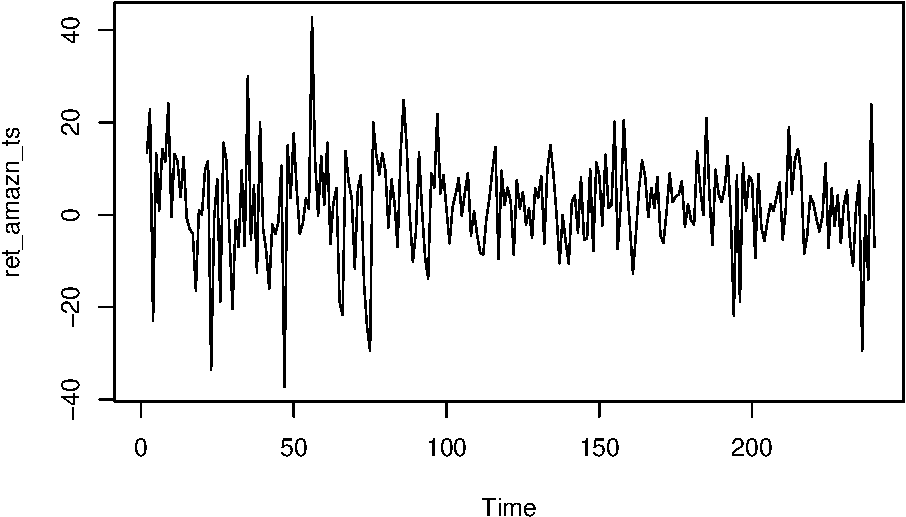
\includegraphics{07-PE_Univariados_files/figure-latex/unnamed-chunk-6-1.pdf}

Dado que queremos saber si existe un proceso AR(2) en estos cambio
debemos calcularlo. Para ello utilizamos la función lm() que realizará una regresión lineal y veremos la relación de los valores con sus valores pasados en \(t-2\):

\begin{Shaded}
\begin{Highlighting}[]
\NormalTok{priceopen}\OtherTok{\textless{}{-}}\NormalTok{data\_precio\_amzn}\SpecialCharTok{$}\NormalTok{price.open}
\NormalTok{priceopen\_amazn}\OtherTok{\textless{}{-}}\FunctionTok{as.data.frame}\NormalTok{(priceopen)}
\NormalTok{priceopen\_amazn}\SpecialCharTok{$}\NormalTok{priceopen\_lag1}\OtherTok{\textless{}{-}}\FunctionTok{lag}\NormalTok{(priceopen\_amazn}\SpecialCharTok{$}\NormalTok{priceopen,}\DecValTok{1}\NormalTok{)}
\NormalTok{priceopen\_amazn}\SpecialCharTok{$}\NormalTok{priceopen\_lag2}\OtherTok{\textless{}{-}}\FunctionTok{lag}\NormalTok{(priceopen\_amazn}\SpecialCharTok{$}\NormalTok{priceopen,}\DecValTok{2}\NormalTok{)}
\NormalTok{ar2\_amazn}\OtherTok{\textless{}{-}}\FunctionTok{lm}\NormalTok{(priceopen}\SpecialCharTok{\textasciitilde{}}\NormalTok{priceopen\_lag1}\SpecialCharTok{+}\NormalTok{priceopen\_lag2, }\AttributeTok{data=}\NormalTok{priceopen\_amazn)}
\end{Highlighting}
\end{Shaded}

Veamos la tabla de la regresión lineal:

\begin{Shaded}
\begin{Highlighting}[]
\FunctionTok{stargazer}\NormalTok{(}
\NormalTok{  ar2\_amazn,}
  \AttributeTok{type =} \StringTok{"html"}\NormalTok{,}
  \AttributeTok{notes.align =} \StringTok{"l"}\NormalTok{, }\AttributeTok{style=}\StringTok{"all"}\NormalTok{, }\AttributeTok{notes.append =} \ConstantTok{FALSE}\NormalTok{,}\AttributeTok{star.char=}\FunctionTok{c}\NormalTok{(}\StringTok{"*"}\NormalTok{), }\AttributeTok{notes=}\FunctionTok{c}\NormalTok{(}\StringTok{"(p\textless{}0.1)=[*], (p\textless{}0.05)=[**], (p\textless{}0.01)=[***]"}\NormalTok{), }\AttributeTok{title =}\StringTok{"AR(2) de los precios de apertura de AMZN"}\NormalTok{, }\AttributeTok{label =} \StringTok{"tab:Ar2precios"}\NormalTok{)}
\end{Highlighting}
\end{Shaded}

AR(2) de los precios de apertura de AMZN

Dependent variable:

priceopen

priceopen\_lag1

0.840***

(0.065)

t = 12.968

p = 0.000

priceopen\_lag2

0.161**

(0.065)

t = 2.468

p = 0.015

Constant

0.580

(0.460)

t = 1.261

p = 0.209

Observations

238

R2

0.988

Adjusted R2

0.987

Residual Std. Error

5.696 (df = 235)

F Statistic

9,358.762*** (df = 2; 235) (p = 0.000)

Note:

(p\textless0.1)={[}*{]}, (p\textless0.05)={[}**{]}, (p\textless0.01)={[}***{]}

La Tabla anterior claramente indica que \textbf{hay una
relación entre el valor del precio y sus valores anteriores en un
proceso AR(2)}.

  \bibliography{book.bib,packages.bib}

\end{document}
